\documentclass[a4paper,11pt]{article}

\frenchspacing
%\usepackage[finnish]{babel}
%\usepackage[utf8x]{inputenc}
\usepackage{graphicx}
\graphicspath{{img/}}
\usepackage{tikz}
%\usepackage[T1]{fontenc}
\usepackage{url}
\usepackage{cite}
\usepackage{hyperref}
\usepackage{amsmath}
\usepackage{dirtree, array}
\usepackage{appendix}
\usepackage[ddmmyyyy]{datetime}
\renewcommand{\dateseparator}{.}
%\usepackage[sorting=none]{biblatex}
\usepackage{./placeins/placeins} % prevents the floats from passing a FloatBarrier
%% Define a new 'leo' style for the package that will use a smaller font.
\makeatletter
\def\url@leostyle{%
  \@ifundefined{selectfont}{\def\UrlFont{\sf}}{\def\UrlFont{\small\ttfamily}}}
\makeatother
%% Now actually use the newly defined style.
\urlstyle{leo}
\begin{document}

\begin{titlepage}
\pagestyle{empty}
\begin{center}

\vspace*{3cm}
\noindent\LARGE{\textbf{
%
%*******************************************************
%Title:
Polygraph implementation using Arduino microcontroller board
%*******************************************************
%
}}
\\
\vspace*{1cm}
\large{
\begin{tabular}{l l}
%
%*******************************************************
%Author:
Henrik Lindblom & 67558R \\
Anne Vainio & 66535U \\
Aki Kauppinen & 12345A
%*******************************************************
%
\end{tabular}

\vspace*{1cm}
\begin{tabular}{l l}
Date & \textbf{
%
%*******************************************************
% Date
\today 
%*******************************************************
%
}
\end{tabular}
}
\end{center}
\end{titlepage}
%kansilehti loppuu 
\pagenumbering{roman}
\tableofcontents
\newpage
\pagenumbering{arabic}
%Varsinainan selkkari alkaa
\section{General}
\begin{figure}[htb]
  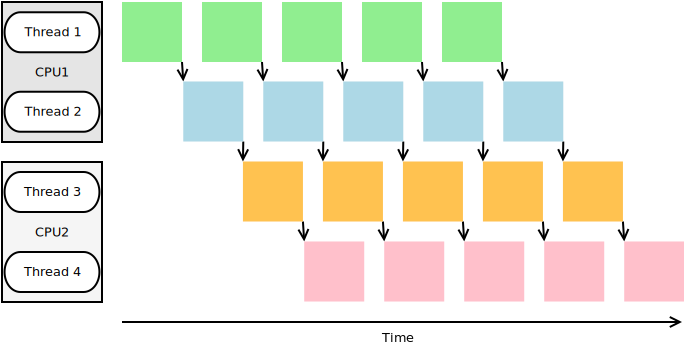
\includegraphics[width=\textwidth]{pipelining2}
  %% \centering
  %% \def\svgwidth{\columnwidth}
  %% %LaTeX with PSTricks extensions
%%Creator: 0.48.2
%%Please note this file requires PSTricks extensions
\psset{xunit=.5pt,yunit=.5pt,runit=.5pt}
\begin{pspicture}(1240.1574707,637.79528809)
{
\newrgbcolor{curcolor}{0.89803922 0.89803922 0.89803922}
\pscustom[linestyle=none,fillstyle=solid,fillcolor=curcolor]
{
\newpath
\moveto(3.62619143,628.03046386)
\lineto(184.93576318,628.03046386)
\lineto(184.93576318,374.19706342)
\lineto(3.62619143,374.19706342)
\closepath
}
}
{
\newrgbcolor{curcolor}{0 0 0}
\pscustom[linewidth=3.62619143,linecolor=curcolor]
{
\newpath
\moveto(3.62619143,628.03046386)
\lineto(184.93576318,628.03046386)
\lineto(184.93576318,374.19706342)
\lineto(3.62619143,374.19706342)
\closepath
}
}
{
\newrgbcolor{curcolor}{0.96078432 0.96078432 0.96078432}
\pscustom[linestyle=none,fillstyle=solid,fillcolor=curcolor]
{
\newpath
\moveto(3.62619143,337.93514908)
\lineto(184.93576318,337.93514908)
\lineto(184.93576318,84.10174864)
\lineto(3.62619143,84.10174864)
\closepath
}
}
{
\newrgbcolor{curcolor}{0 0 0}
\pscustom[linewidth=3.62619143,linecolor=curcolor]
{
\newpath
\moveto(3.62619143,337.93514908)
\lineto(184.93576318,337.93514908)
\lineto(184.93576318,84.10174864)
\lineto(3.62619143,84.10174864)
\closepath
}
}
{
\newrgbcolor{curcolor}{0 0 0}
\pscustom[linewidth=3.62619143,linecolor=curcolor]
{
\newpath
\moveto(329.98342057,519.24472082)
\lineto(331.77477109,491.98119587)
}
}
{
\newrgbcolor{curcolor}{0 0 0}
\pscustom[linewidth=3.62619143,linecolor=curcolor]
{
\newpath
\moveto(321.80635888,505.43255764)
\lineto(332.04128421,487.93437087)
\lineto(339.89742795,506.62194843)
}
}
{
\newrgbcolor{curcolor}{0 0 0}
\pscustom[linewidth=3.62619143,linecolor=curcolor]
{
\newpath
\moveto(441.09174985,375.10361128)
\lineto(440.60400453,346.94806294)
}
}
{
\newrgbcolor{curcolor}{0 0 0}
\pscustom[linewidth=3.62619143,linecolor=curcolor]
{
\newpath
\moveto(431.78330581,361.18084927)
\lineto(440.53330574,342.89577896)
\lineto(449.91244989,360.86718371)
}
}
{
\newrgbcolor{curcolor}{0 0 0}
\pscustom[linewidth=3.62619143,linecolor=curcolor]
{
\newpath
\moveto(549.25014672,230.05595389)
\lineto(551.05416811,201.88590875)
}
}
{
\newrgbcolor{curcolor}{0 0 0}
\pscustom[linewidth=3.62619143,linecolor=curcolor]
{
\newpath
\moveto(541.10753828,215.35356072)
\lineto(551.31345408,197.83905609)
\lineto(559.20042045,216.51394198)
}
}
{
\newrgbcolor{curcolor}{0 0 0}
\pscustom[linewidth=3.62619143,linecolor=curcolor]
{
\newpath
\moveto(475.03107796,519.24472082)
\lineto(476.82242848,491.98119587)
}
}
{
\newrgbcolor{curcolor}{0 0 0}
\pscustom[linewidth=3.62619143,linecolor=curcolor]
{
\newpath
\moveto(466.85401627,505.43255764)
\lineto(477.0889416,487.93437087)
\lineto(484.94508534,506.62194843)
}
}
{
\newrgbcolor{curcolor}{0 0 0}
\pscustom[linewidth=3.62619143,linecolor=curcolor]
{
\newpath
\moveto(586.13940724,375.10361128)
\lineto(585.65166192,346.94806294)
}
}
{
\newrgbcolor{curcolor}{0 0 0}
\pscustom[linewidth=3.62619143,linecolor=curcolor]
{
\newpath
\moveto(576.8309632,361.18084927)
\lineto(585.58096314,342.89577896)
\lineto(594.96010728,360.86718371)
}
}
{
\newrgbcolor{curcolor}{0 0 0}
\pscustom[linewidth=3.62619143,linecolor=curcolor]
{
\newpath
\moveto(694.29780412,230.05595389)
\lineto(696.1018255,201.88590875)
}
}
{
\newrgbcolor{curcolor}{0 0 0}
\pscustom[linewidth=3.62619143,linecolor=curcolor]
{
\newpath
\moveto(686.15519568,215.35356072)
\lineto(696.36111147,197.83905609)
\lineto(704.24807784,216.51394198)
}
}
{
\newrgbcolor{curcolor}{0 0 0}
\pscustom[linewidth=3.62619143,linecolor=curcolor]
{
\newpath
\moveto(620.07873535,519.24472082)
\lineto(621.87008587,491.98119587)
}
}
{
\newrgbcolor{curcolor}{0 0 0}
\pscustom[linewidth=3.62619143,linecolor=curcolor]
{
\newpath
\moveto(611.90167367,505.43255764)
\lineto(622.13659899,487.93437087)
\lineto(629.99274273,506.62194843)
}
}
{
\newrgbcolor{curcolor}{0 0 0}
\pscustom[linewidth=3.62619143,linecolor=curcolor]
{
\newpath
\moveto(731.18706463,375.10361128)
\lineto(730.69931931,346.94806294)
}
}
{
\newrgbcolor{curcolor}{0 0 0}
\pscustom[linewidth=3.62619143,linecolor=curcolor]
{
\newpath
\moveto(721.8786206,361.18084927)
\lineto(730.62862053,342.89577896)
\lineto(740.00776467,360.86718371)
}
}
{
\newrgbcolor{curcolor}{0 0 0}
\pscustom[linewidth=3.62619143,linecolor=curcolor]
{
\newpath
\moveto(839.34546151,230.05595389)
\lineto(841.14948289,201.88590875)
}
}
{
\newrgbcolor{curcolor}{0 0 0}
\pscustom[linewidth=3.62619143,linecolor=curcolor]
{
\newpath
\moveto(831.20285307,215.35356072)
\lineto(841.40876886,197.83905609)
\lineto(849.29573523,216.51394198)
}
}
{
\newrgbcolor{curcolor}{0 0 0}
\pscustom[linewidth=3.62619143,linecolor=curcolor]
{
\newpath
\moveto(765.12639274,519.24472082)
\lineto(766.91774326,491.98119587)
}
}
{
\newrgbcolor{curcolor}{0 0 0}
\pscustom[linewidth=3.62619143,linecolor=curcolor]
{
\newpath
\moveto(756.94933106,505.43255764)
\lineto(767.18425638,487.93437087)
\lineto(775.04040013,506.62194843)
}
}
{
\newrgbcolor{curcolor}{0 0 0}
\pscustom[linewidth=3.62619143,linecolor=curcolor]
{
\newpath
\moveto(876.23472203,375.10361128)
\lineto(875.7469767,346.94806294)
}
}
{
\newrgbcolor{curcolor}{0 0 0}
\pscustom[linewidth=3.62619143,linecolor=curcolor]
{
\newpath
\moveto(866.92627799,361.18084927)
\lineto(875.67627792,342.89577896)
\lineto(885.05542207,360.86718371)
}
}
{
\newrgbcolor{curcolor}{0 0 0}
\pscustom[linewidth=3.62619143,linecolor=curcolor]
{
\newpath
\moveto(984.3931189,230.05595389)
\lineto(986.19714029,201.88590875)
}
}
{
\newrgbcolor{curcolor}{0 0 0}
\pscustom[linewidth=3.62619143,linecolor=curcolor]
{
\newpath
\moveto(976.25051046,215.35356072)
\lineto(986.45642625,197.83905609)
\lineto(994.34339262,216.51394198)
}
}
{
\newrgbcolor{curcolor}{0 0 0}
\pscustom[linewidth=3.62619143,linecolor=curcolor]
{
\newpath
\moveto(910.17405014,519.24472082)
\lineto(911.96540066,491.98119587)
}
}
{
\newrgbcolor{curcolor}{0 0 0}
\pscustom[linewidth=3.62619143,linecolor=curcolor]
{
\newpath
\moveto(901.99698845,505.43255764)
\lineto(912.23191378,487.93437087)
\lineto(920.08805752,506.62194843)
}
}
{
\newrgbcolor{curcolor}{0 0 0}
\pscustom[linewidth=3.62619143,linecolor=curcolor]
{
\newpath
\moveto(1021.28237942,375.10361128)
\lineto(1020.79468943,346.94806294)
}
}
{
\newrgbcolor{curcolor}{0 0 0}
\pscustom[linewidth=3.62619143,linecolor=curcolor]
{
\newpath
\moveto(1011.97393538,361.18084927)
\lineto(1020.72393531,342.89577896)
\lineto(1030.10307946,360.86718371)
}
}
{
\newrgbcolor{curcolor}{0 0 0}
\pscustom[linewidth=3.62619143,linecolor=curcolor]
{
\newpath
\moveto(1129.44077629,230.05595389)
\lineto(1131.24479768,201.88590875)
}
}
{
\newrgbcolor{curcolor}{0 0 0}
\pscustom[linewidth=3.62619143,linecolor=curcolor]
{
\newpath
\moveto(1121.29816785,215.35356072)
\lineto(1131.50408365,197.83905609)
\lineto(1139.39105002,216.51394198)
}
}
{
\newrgbcolor{curcolor}{0 0 0}
\pscustom[linestyle=none,fillstyle=solid,fillcolor=curcolor]
{
\newpath
\moveto(698.6196814,11.57791994)
\lineto(698.6196814,26.22977068)
\lineto(693.14648426,26.22977068)
\lineto(693.14648426,28.19014978)
\lineto(706.31388608,28.19014978)
\lineto(706.31388608,26.22977068)
\lineto(700.8180256,26.22977068)
\lineto(700.8180256,11.57791994)
\closepath
}
}
{
\newrgbcolor{curcolor}{0 0 0}
\pscustom[linestyle=none,fillstyle=solid,fillcolor=curcolor]
{
\newpath
\moveto(708.33092364,25.84449386)
\lineto(708.33092364,28.19014978)
\lineto(710.37062443,28.19014978)
\lineto(710.37062443,25.84449386)
\closepath
\moveto(708.33092364,11.57791994)
\lineto(708.33092364,23.61215465)
\lineto(710.37062443,23.61215465)
\lineto(710.37062443,11.57791994)
\closepath
}
}
{
\newrgbcolor{curcolor}{0 0 0}
\pscustom[linestyle=none,fillstyle=solid,fillcolor=curcolor]
{
\newpath
\moveto(713.48683418,11.57791994)
\lineto(713.48683418,23.61215465)
\lineto(715.31123323,23.61215465)
\lineto(715.31123323,21.92373566)
\curveto(715.68895187,22.51297162)(716.19132212,22.98701272)(716.81834549,23.34586038)
\curveto(717.44535913,23.70468451)(718.1592537,23.88410245)(718.96003132,23.88411476)
\curveto(719.85144822,23.88410245)(720.58234028,23.69901868)(721.15270968,23.32886288)
\curveto(721.7230607,22.95868357)(722.12533462,22.44120444)(722.35953266,21.77642394)
\curveto(723.31138167,23.18153955)(724.55030981,23.88410245)(726.07632078,23.88411476)
\curveto(727.26990815,23.88410245)(728.18777259,23.55359571)(728.82991685,22.89259354)
\curveto(729.47202737,22.23156874)(729.79309106,21.21360797)(729.7931089,19.83870818)
\lineto(729.7931089,11.57791994)
\lineto(727.76473977,11.57791994)
\lineto(727.76473977,19.15880791)
\curveto(727.76472396,19.97467983)(727.69862261,20.56203753)(727.56643553,20.92088277)
\curveto(727.43421722,21.27970932)(727.19436375,21.56866664)(726.84687441,21.78775561)
\curveto(726.49935529,22.00682415)(726.09141554,22.11636353)(725.62305393,22.11637407)
\curveto(724.776943,22.11636353)(724.0743801,21.83496065)(723.51536311,21.27216457)
\curveto(722.956323,20.70934911)(722.67680873,19.80848216)(722.67681945,18.56956101)
\lineto(722.67681945,11.57791994)
\lineto(720.63711865,11.57791994)
\lineto(720.63711865,19.396773)
\curveto(720.63710997,20.30329797)(720.47091229,20.98319755)(720.13852512,21.4364738)
\curveto(719.80612158,21.88973033)(719.26220192,22.11636353)(718.50676448,22.11637407)
\curveto(717.9326205,22.11636353)(717.4019211,21.96527473)(716.91466469,21.66310722)
\curveto(716.42739836,21.36091955)(716.0742283,20.91898481)(715.85515344,20.33730171)
\curveto(715.63607079,19.75560108)(715.52653141,18.91705825)(715.52653498,17.82167072)
\lineto(715.52653498,11.57791994)
\closepath
}
}
{
\newrgbcolor{curcolor}{0 0 0}
\pscustom[linestyle=none,fillstyle=solid,fillcolor=curcolor]
{
\newpath
\moveto(741.07945361,15.45335146)
\lineto(743.18714443,15.19272302)
\curveto(742.85473721,13.96134571)(742.23905036,13.00570907)(741.34008205,12.32581024)
\curveto(740.44109367,11.6459099)(739.29281882,11.30596011)(737.89525403,11.30595984)
\curveto(736.13506296,11.30596011)(734.7393802,11.84799117)(733.70820156,12.93205464)
\curveto(732.67701812,14.0161154)(732.1614276,15.53644642)(732.16142845,17.49305226)
\curveto(732.1614276,19.51763622)(732.68268395,21.08895971)(733.72519906,22.20702744)
\curveto(734.76770935,23.32507391)(736.11995408,23.88410245)(737.78193732,23.88411476)
\curveto(739.39102654,23.88410245)(740.70549907,23.33640557)(741.72535886,22.24102245)
\curveto(742.74519783,21.14561801)(743.25512252,19.60451228)(743.25513446,17.61770064)
\curveto(743.25512252,17.49682356)(743.2513453,17.31551701)(743.24380279,17.07378043)
\lineto(734.26911928,17.07378043)
\curveto(734.34466072,15.75174796)(734.71860549,14.73945302)(735.39095472,14.03689257)
\curveto(736.06329578,13.33432721)(736.90183861,12.98304575)(737.9065857,12.98304716)
\curveto(738.65446865,12.98304575)(739.29281882,13.17946119)(739.82163812,13.57229406)
\curveto(740.3504404,13.96512293)(740.76971181,14.59214144)(741.07945361,15.45335146)
\closepath
\moveto(734.38243599,18.75086775)
\lineto(741.10211695,18.75086775)
\curveto(741.01145388,19.76315552)(740.75460293,20.52237672)(740.33156332,21.02853364)
\curveto(739.68187247,21.81418594)(738.83955243,22.20701681)(737.80460066,22.20702744)
\curveto(736.86784363,22.20701681)(736.08029327,21.89350755)(735.44194724,21.26649874)
\curveto(734.80359294,20.63947054)(734.45042288,19.80092772)(734.38243599,18.75086775)
\closepath
}
}
{
\newrgbcolor{curcolor}{1 1 1}
\pscustom[linestyle=none,fillstyle=solid,fillcolor=curcolor]
{
\newpath
\moveto(36.94182524,319.8041919)
\lineto(151.62012937,319.8041919)
\curveto(167.45389427,319.8041919)(180.2897054,303.56973285)(180.2897054,283.54227755)
\curveto(180.2897054,263.51482226)(167.45389427,247.28036321)(151.62012937,247.28036321)
\lineto(36.94182524,247.28036321)
\curveto(21.10806034,247.28036321)(8.27224921,263.51482226)(8.27224921,283.54227755)
\curveto(8.27224921,303.56973285)(21.10806034,319.8041919)(36.94182524,319.8041919)
\closepath
}
}
{
\newrgbcolor{curcolor}{0 0 0}
\pscustom[linewidth=3.62619143,linecolor=curcolor]
{
\newpath
\moveto(36.94182524,319.8041919)
\lineto(151.62012937,319.8041919)
\curveto(167.45389427,319.8041919)(180.2897054,303.56973285)(180.2897054,283.54227755)
\curveto(180.2897054,263.51482226)(167.45389427,247.28036321)(151.62012937,247.28036321)
\lineto(36.94182524,247.28036321)
\curveto(21.10806034,247.28036321)(8.27224921,263.51482226)(8.27224921,283.54227755)
\curveto(8.27224921,303.56973285)(21.10806034,319.8041919)(36.94182524,319.8041919)
}
}
{
\newrgbcolor{curcolor}{0 0 0}
\pscustom[linestyle=none,fillstyle=solid,fillcolor=curcolor]
{
\newpath
\moveto(53.8155798,276.28989468)
\lineto(53.8155798,290.94174542)
\lineto(48.34238266,290.94174542)
\lineto(48.34238266,292.90212452)
\lineto(61.50978448,292.90212452)
\lineto(61.50978448,290.94174542)
\lineto(56.01392399,290.94174542)
\lineto(56.01392399,276.28989468)
\closepath
}
}
{
\newrgbcolor{curcolor}{0 0 0}
\pscustom[linestyle=none,fillstyle=solid,fillcolor=curcolor]
{
\newpath
\moveto(63.51549036,276.28989468)
\lineto(63.51549036,292.90212452)
\lineto(65.55519116,292.90212452)
\lineto(65.55519116,286.94166552)
\curveto(66.50704701,288.04460309)(67.70820295,288.59607719)(69.15866257,288.5960895)
\curveto(70.0500793,288.59607719)(70.82440938,288.42043647)(71.48165515,288.06916679)
\curveto(72.13888192,287.71787356)(72.6091458,287.2325008)(72.8924482,286.61304706)
\curveto(73.17572879,285.99357267)(73.31737453,285.09459433)(73.31738586,283.91610934)
\lineto(73.31738586,276.28989468)
\lineto(71.27768507,276.28989468)
\lineto(71.27768507,283.91610934)
\curveto(71.27767577,284.93595109)(71.05670841,285.6781748)(70.61478231,286.14278271)
\curveto(70.17283895,286.6073709)(69.54770905,286.83966993)(68.73939074,286.83968048)
\curveto(68.1350288,286.83966993)(67.5665572,286.6829153)(67.03397424,286.36941613)
\curveto(66.50138118,286.0558968)(66.12177058,285.63095955)(65.89514129,285.09460313)
\curveto(65.66850419,284.5582291)(65.55518759,283.81789399)(65.55519116,282.87359559)
\lineto(65.55519116,276.28989468)
\closepath
}
}
{
\newrgbcolor{curcolor}{0 0 0}
\pscustom[linestyle=none,fillstyle=solid,fillcolor=curcolor]
{
\newpath
\moveto(76.4109317,276.28989468)
\lineto(76.4109317,288.32412939)
\lineto(78.24666242,288.32412939)
\lineto(78.24666242,286.49973035)
\curveto(78.71503435,287.35337184)(79.14752603,287.91617761)(79.54413876,288.18814934)
\curveto(79.94074221,288.46009728)(80.37701111,288.59607719)(80.85294677,288.5960895)
\curveto(81.54039485,288.59607719)(82.23918053,288.37699844)(82.94930593,287.93885258)
\lineto(82.24674232,286.0464635)
\curveto(81.74814194,286.3410769)(81.24954891,286.48838848)(80.75096173,286.48839868)
\curveto(80.30524393,286.48838848)(79.90485862,286.35429717)(79.5498046,286.08612435)
\curveto(79.19474128,285.81793194)(78.94166754,285.44587578)(78.79058263,284.96995475)
\curveto(78.56394555,284.24471984)(78.45062895,283.45150366)(78.4506325,282.59030382)
\lineto(78.4506325,276.28989468)
\closepath
}
}
{
\newrgbcolor{curcolor}{0 0 0}
\pscustom[linestyle=none,fillstyle=solid,fillcolor=curcolor]
{
\newpath
\moveto(92.4225824,280.1653262)
\lineto(94.53027322,279.90469777)
\curveto(94.19786599,278.67332046)(93.58217915,277.71768382)(92.68321083,277.03778498)
\curveto(91.78422246,276.35788464)(90.6359476,276.01793485)(89.23838282,276.01793458)
\curveto(87.47819175,276.01793485)(86.08250899,276.55996591)(85.05133034,277.64402938)
\curveto(84.02014691,278.72809014)(83.50455639,280.24842116)(83.50455724,282.205027)
\curveto(83.50455639,284.22961096)(84.02581274,285.80093445)(85.06832785,286.91900218)
\curveto(86.11083814,288.03704865)(87.46308287,288.59607719)(89.12506611,288.5960895)
\curveto(90.73415532,288.59607719)(92.04862786,288.04838031)(93.06848765,286.95299719)
\curveto(94.08832661,285.85759275)(94.5982513,284.31648702)(94.59826325,282.32967538)
\curveto(94.5982513,282.2087983)(94.59447408,282.02749175)(94.58693158,281.78575517)
\lineto(85.61224806,281.78575517)
\curveto(85.68778951,280.4637227)(86.06173428,279.45142776)(86.7340835,278.74886731)
\curveto(87.40642457,278.04630195)(88.24496739,277.6950205)(89.24971449,277.6950219)
\curveto(89.99759744,277.6950205)(90.6359476,277.89143593)(91.1647669,278.2842688)
\curveto(91.69356918,278.67709768)(92.11284059,279.30411618)(92.4225824,280.1653262)
\closepath
\moveto(85.72556478,283.46284249)
\lineto(92.44524574,283.46284249)
\curveto(92.35458267,284.47513026)(92.09773172,285.23435146)(91.6746921,285.74050838)
\curveto(91.02500126,286.52616068)(90.18268121,286.91899155)(89.14772945,286.91900218)
\curveto(88.21097241,286.91899155)(87.42342206,286.60548229)(86.78507602,285.97847348)
\curveto(86.14672173,285.35144528)(85.79355166,284.51290246)(85.72556478,283.46284249)
\closepath
}
}
{
\newrgbcolor{curcolor}{0 0 0}
\pscustom[linestyle=none,fillstyle=solid,fillcolor=curcolor]
{
\newpath
\moveto(104.95541199,277.7743436)
\curveto(104.19995862,277.13221473)(103.47284379,276.67894834)(102.7740653,276.41454307)
\curveto(102.07527242,276.15013755)(101.32549426,276.01793485)(100.52472859,276.01793458)
\curveto(99.20269666,276.01793485)(98.1866245,276.34088715)(97.47650906,276.98679246)
\curveto(96.76638981,277.63269637)(96.41133114,278.45801892)(96.41133198,279.46276259)
\curveto(96.41133114,280.05200573)(96.54542245,280.59025957)(96.8136063,281.07752572)
\curveto(97.08178768,281.56478231)(97.43306913,281.95572457)(97.86745172,282.25035368)
\curveto(98.30182971,282.54497088)(98.79097969,282.76782685)(99.33490312,282.91892228)
\curveto(99.73528467,283.02467781)(100.33963986,283.12666275)(101.1479705,283.2248774)
\curveto(102.79483281,283.4212859)(104.00732041,283.65547353)(104.78543692,283.92744101)
\curveto(104.79298215,284.20694764)(104.79675937,284.38447698)(104.79676859,284.46002955)
\curveto(104.79675937,285.29100976)(104.60412115,285.87647885)(104.21885337,286.21643857)
\curveto(103.69758837,286.67724947)(102.92325829,286.90765989)(101.89586079,286.90767051)
\curveto(100.93644061,286.90765989)(100.22821187,286.7395736)(99.77117246,286.40341114)
\curveto(99.31412465,286.06722846)(98.97606347,285.47231632)(98.7569879,284.61867294)
\lineto(96.76261378,284.89063305)
\curveto(96.94391915,285.74427615)(97.24231952,286.43361879)(97.6578158,286.95866303)
\curveto(98.07330791,287.48368593)(98.67388587,287.88784846)(99.45955151,288.17115183)
\curveto(100.24520936,288.45443145)(101.15551936,288.59607719)(102.19048424,288.5960895)
\curveto(103.21788144,288.59607719)(104.05264705,288.47520616)(104.69478355,288.23347603)
\curveto(105.33690182,287.99172201)(105.80905431,287.6876558)(106.11124244,287.3212765)
\curveto(106.4134095,286.95487514)(106.62493381,286.4921657)(106.74581602,285.93314679)
\curveto(106.81379481,285.58563292)(106.84778979,284.95861441)(106.84780106,284.05208939)
\lineto(106.84780106,281.33248832)
\curveto(106.84778979,279.43631888)(106.89122782,278.23705155)(106.97811528,277.73468275)
\curveto(107.06497993,277.23231105)(107.23684344,276.75071551)(107.49370632,276.28989468)
\lineto(105.36335215,276.28989468)
\curveto(105.15181804,276.71294332)(105.01583813,277.20775913)(104.95541199,277.7743436)
\closepath
\moveto(104.78543692,282.32967538)
\curveto(104.04509261,282.02749175)(102.93458995,281.77064079)(101.45392562,281.55912175)
\curveto(100.61537691,281.43824544)(100.02235339,281.30226552)(99.67485326,281.15118159)
\curveto(99.32734492,281.00008793)(99.05916231,280.77912056)(98.87030461,280.48827883)
\curveto(98.68144031,280.19742869)(98.58700982,279.87447639)(98.58701283,279.51942095)
\curveto(98.58700982,278.97549805)(98.7928683,278.52223166)(99.20458891,278.15962042)
\curveto(99.61630225,277.79700543)(100.21876882,277.61569888)(101.01199045,277.6157002)
\curveto(101.79764675,277.61569888)(102.49643244,277.78756238)(103.1083496,278.13129124)
\curveto(103.72025169,278.47501641)(104.16974086,278.94528029)(104.45681846,279.54208429)
\curveto(104.67588833,280.00290187)(104.78542771,280.68280145)(104.78543692,281.58178509)
\closepath
}
}
{
\newrgbcolor{curcolor}{0 0 0}
\pscustom[linestyle=none,fillstyle=solid,fillcolor=curcolor]
{
\newpath
\moveto(117.82818826,276.28989468)
\lineto(117.82818826,277.80833861)
\curveto(117.0651805,276.6147356)(115.94334618,276.01793485)(114.46268194,276.01793458)
\curveto(113.50326211,276.01793485)(112.62128126,276.28234024)(111.81673674,276.81115155)
\curveto(111.01218557,277.33996182)(110.38894428,278.07840832)(109.94701101,279.02649326)
\curveto(109.50507482,279.97457272)(109.28410745,281.06430067)(109.28410825,282.29568037)
\curveto(109.28410745,283.4968303)(109.48430011,284.58655825)(109.88468682,285.56486748)
\curveto(110.28507073,286.54315817)(110.8856487,287.29293632)(111.68642252,287.81420419)
\curveto(112.48718995,288.33544902)(113.38239107,288.59607719)(114.37202857,288.5960895)
\curveto(115.09724892,288.59607719)(115.74315352,288.44309979)(116.30974433,288.13715682)
\curveto(116.8763195,287.83119016)(117.33714033,287.43269346)(117.6922082,286.94166552)
\lineto(117.6922082,292.90212452)
\lineto(119.72057733,292.90212452)
\lineto(119.72057733,276.28989468)
\closepath
\moveto(111.3804674,282.29568037)
\curveto(111.38046451,280.75456863)(111.70530542,279.60251656)(112.35499112,278.83952068)
\curveto(113.00466908,278.07651971)(113.77144472,277.6950205)(114.65532035,277.6950219)
\curveto(115.54673809,277.6950205)(116.30407068,278.05952222)(116.9273204,278.78852816)
\curveto(117.55055326,279.51752911)(117.8621739,280.62992038)(117.86218327,282.1257053)
\curveto(117.8621739,283.77256735)(117.54488743,284.98127773)(116.9103229,285.75184005)
\curveto(116.27574153,286.52238346)(115.49385701,286.90765989)(114.56466698,286.90767051)
\curveto(113.65812812,286.90765989)(112.90079553,286.53749234)(112.29266692,285.79716674)
\curveto(111.68453071,285.05682213)(111.38046451,283.88966117)(111.3804674,282.29568037)
\closepath
}
}
{
\newrgbcolor{curcolor}{0 0 0}
\pscustom[linestyle=none,fillstyle=solid,fillcolor=curcolor]
{
\newpath
\moveto(128.81990606,280.6752514)
\lineto(130.85960686,280.94721151)
\curveto(131.09379148,279.79137755)(131.49228818,278.95850056)(132.05509816,278.44857803)
\curveto(132.61789972,277.93865118)(133.30346514,277.68368884)(134.11179647,277.68369023)
\curveto(135.07120406,277.68368884)(135.88141773,278.01608419)(136.54243992,278.68087729)
\curveto(137.20344471,279.3456656)(137.53395145,280.16909955)(137.53396114,281.15118159)
\curveto(137.53395145,282.08792727)(137.22799664,282.86036874)(136.61609578,283.46850833)
\curveto(136.00417738,284.07663356)(135.22607008,284.38069976)(134.28177153,284.38070785)
\curveto(133.89648866,284.38069976)(133.41678173,284.30515536)(132.8426493,284.15407443)
\lineto(133.06928273,285.94447846)
\curveto(133.20525742,285.92935993)(133.3147968,285.92180549)(133.39790119,285.92181512)
\curveto(134.26665622,285.92180549)(135.04854074,286.14843868)(135.74355711,286.60171539)
\curveto(136.43855767,287.05497147)(136.78606191,287.75375715)(136.78607085,288.69807454)
\curveto(136.78606191,289.44595168)(136.53298817,290.06541574)(136.02684888,290.5564686)
\curveto(135.52069323,291.04749292)(134.86723419,291.29301222)(134.06646978,291.29302722)
\curveto(133.27324738,291.29301222)(132.61223389,291.04371571)(132.08342734,290.54513693)
\curveto(131.55461231,290.04652965)(131.21466252,289.2986401)(131.06357694,288.30146605)
\lineto(129.02387614,288.66407953)
\curveto(129.27317148,290.03142077)(129.83975447,291.09093095)(130.72362681,291.84261327)
\curveto(131.60749339,292.59426448)(132.70666439,292.97009787)(134.0211431,292.97011455)
\curveto(134.9276697,292.97009787)(135.76243531,292.77557104)(136.52544241,292.38653348)
\curveto(137.28843216,291.99746374)(137.87201263,291.46676434)(138.2761856,290.79443369)
\curveto(138.6803377,290.12207404)(138.88241896,289.40817948)(138.88243,288.65274786)
\curveto(138.88241896,287.93506371)(138.68978075,287.28160466)(138.30451477,286.69236876)
\curveto(137.91922788,286.10311205)(137.34886767,285.63473677)(136.59343244,285.28724154)
\curveto(137.57550087,285.06059935)(138.33849929,284.59033547)(138.88243,283.87644849)
\curveto(139.42633863,283.16254633)(139.69829847,282.26923382)(139.69831032,281.19650827)
\curveto(139.69829847,279.74605091)(139.16948768,278.51656583)(138.11187637,277.50804933)
\curveto(137.05424452,276.49953039)(135.71710867,275.99527153)(134.1004648,275.99527124)
\curveto(132.64245165,275.99527153)(131.43185266,276.42965182)(130.46866421,277.29841341)
\curveto(129.5054705,278.16717299)(128.955885,279.29278452)(128.81990606,280.6752514)
\closepath
}
}
{
\newrgbcolor{curcolor}{1 1 1}
\pscustom[linestyle=none,fillstyle=solid,fillcolor=curcolor]
{
\newpath
\moveto(36.94182524,174.75653451)
\lineto(151.62012937,174.75653451)
\curveto(167.45389427,174.75653451)(180.2897054,158.52207546)(180.2897054,138.49462016)
\curveto(180.2897054,118.46716487)(167.45389427,102.23270581)(151.62012937,102.23270581)
\lineto(36.94182524,102.23270581)
\curveto(21.10806034,102.23270581)(8.27224921,118.46716487)(8.27224921,138.49462016)
\curveto(8.27224921,158.52207546)(21.10806034,174.75653451)(36.94182524,174.75653451)
\closepath
}
}
{
\newrgbcolor{curcolor}{0 0 0}
\pscustom[linewidth=3.62619143,linecolor=curcolor]
{
\newpath
\moveto(36.94182524,174.75653451)
\lineto(151.62012937,174.75653451)
\curveto(167.45389427,174.75653451)(180.2897054,158.52207546)(180.2897054,138.49462016)
\curveto(180.2897054,118.46716487)(167.45389427,102.23270581)(151.62012937,102.23270581)
\lineto(36.94182524,102.23270581)
\curveto(21.10806034,102.23270581)(8.27224921,118.46716487)(8.27224921,138.49462016)
\curveto(8.27224921,158.52207546)(21.10806034,174.75653451)(36.94182524,174.75653451)
}
}
{
\newrgbcolor{curcolor}{0 0 0}
\pscustom[linestyle=none,fillstyle=solid,fillcolor=curcolor]
{
\newpath
\moveto(53.8155798,131.24223729)
\lineto(53.8155798,145.89408803)
\lineto(48.34238266,145.89408803)
\lineto(48.34238266,147.85446713)
\lineto(61.50978448,147.85446713)
\lineto(61.50978448,145.89408803)
\lineto(56.01392399,145.89408803)
\lineto(56.01392399,131.24223729)
\closepath
}
}
{
\newrgbcolor{curcolor}{0 0 0}
\pscustom[linestyle=none,fillstyle=solid,fillcolor=curcolor]
{
\newpath
\moveto(63.51549036,131.24223729)
\lineto(63.51549036,147.85446713)
\lineto(65.55519116,147.85446713)
\lineto(65.55519116,141.89400813)
\curveto(66.50704701,142.99694569)(67.70820295,143.5484198)(69.15866257,143.54843211)
\curveto(70.0500793,143.5484198)(70.82440938,143.37277908)(71.48165515,143.0215094)
\curveto(72.13888192,142.67021617)(72.6091458,142.18484341)(72.8924482,141.56538967)
\curveto(73.17572879,140.94591528)(73.31737453,140.04693693)(73.31738586,138.86845194)
\lineto(73.31738586,131.24223729)
\lineto(71.27768507,131.24223729)
\lineto(71.27768507,138.86845194)
\curveto(71.27767577,139.8882937)(71.05670841,140.63051741)(70.61478231,141.09512532)
\curveto(70.17283895,141.55971351)(69.54770905,141.79201254)(68.73939074,141.79202309)
\curveto(68.1350288,141.79201254)(67.5665572,141.63525791)(67.03397424,141.32175874)
\curveto(66.50138118,141.0082394)(66.12177058,140.58330216)(65.89514129,140.04694574)
\curveto(65.66850419,139.5105717)(65.55518759,138.7702366)(65.55519116,137.8259382)
\lineto(65.55519116,131.24223729)
\closepath
}
}
{
\newrgbcolor{curcolor}{0 0 0}
\pscustom[linestyle=none,fillstyle=solid,fillcolor=curcolor]
{
\newpath
\moveto(76.4109317,131.24223729)
\lineto(76.4109317,143.276472)
\lineto(78.24666242,143.276472)
\lineto(78.24666242,141.45207295)
\curveto(78.71503435,142.30571445)(79.14752603,142.86852022)(79.54413876,143.14049195)
\curveto(79.94074221,143.41243989)(80.37701111,143.5484198)(80.85294677,143.54843211)
\curveto(81.54039485,143.5484198)(82.23918053,143.32934105)(82.94930593,142.89119518)
\lineto(82.24674232,140.99880611)
\curveto(81.74814194,141.29341951)(81.24954891,141.44073109)(80.75096173,141.44074128)
\curveto(80.30524393,141.44073109)(79.90485862,141.30663978)(79.5498046,141.03846696)
\curveto(79.19474128,140.77027455)(78.94166754,140.39821839)(78.79058263,139.92229736)
\curveto(78.56394555,139.19706245)(78.45062895,138.40384627)(78.4506325,137.54264642)
\lineto(78.4506325,131.24223729)
\closepath
}
}
{
\newrgbcolor{curcolor}{0 0 0}
\pscustom[linestyle=none,fillstyle=solid,fillcolor=curcolor]
{
\newpath
\moveto(92.4225824,135.11766881)
\lineto(94.53027322,134.85704037)
\curveto(94.19786599,133.62566306)(93.58217915,132.67002642)(92.68321083,131.99012758)
\curveto(91.78422246,131.31022725)(90.6359476,130.97027746)(89.23838282,130.97027719)
\curveto(87.47819175,130.97027746)(86.08250899,131.51230852)(85.05133034,132.59637199)
\curveto(84.02014691,133.68043275)(83.50455639,135.20076377)(83.50455724,137.15736961)
\curveto(83.50455639,139.18195357)(84.02581274,140.75327706)(85.06832785,141.87134479)
\curveto(86.11083814,142.98939125)(87.46308287,143.5484198)(89.12506611,143.54843211)
\curveto(90.73415532,143.5484198)(92.04862786,143.00072291)(93.06848765,141.9053398)
\curveto(94.08832661,140.80993536)(94.5982513,139.26882963)(94.59826325,137.28201799)
\curveto(94.5982513,137.16114091)(94.59447408,136.97983436)(94.58693158,136.73809778)
\lineto(85.61224806,136.73809778)
\curveto(85.68778951,135.41606531)(86.06173428,134.40377037)(86.7340835,133.70120992)
\curveto(87.40642457,132.99864456)(88.24496739,132.6473631)(89.24971449,132.64736451)
\curveto(89.99759744,132.6473631)(90.6359476,132.84377854)(91.1647669,133.23661141)
\curveto(91.69356918,133.62944028)(92.11284059,134.25645879)(92.4225824,135.11766881)
\closepath
\moveto(85.72556478,138.4151851)
\lineto(92.44524574,138.4151851)
\curveto(92.35458267,139.42747287)(92.09773172,140.18669407)(91.6746921,140.69285099)
\curveto(91.02500126,141.47850328)(90.18268121,141.87133416)(89.14772945,141.87134479)
\curveto(88.21097241,141.87133416)(87.42342206,141.5578249)(86.78507602,140.93081608)
\curveto(86.14672173,140.30378789)(85.79355166,139.46524507)(85.72556478,138.4151851)
\closepath
}
}
{
\newrgbcolor{curcolor}{0 0 0}
\pscustom[linestyle=none,fillstyle=solid,fillcolor=curcolor]
{
\newpath
\moveto(104.95541199,132.72668621)
\curveto(104.19995862,132.08455733)(103.47284379,131.63129094)(102.7740653,131.36688567)
\curveto(102.07527242,131.10248015)(101.32549426,130.97027746)(100.52472859,130.97027719)
\curveto(99.20269666,130.97027746)(98.1866245,131.29322976)(97.47650906,131.93913506)
\curveto(96.76638981,132.58503897)(96.41133114,133.41036153)(96.41133198,134.4151052)
\curveto(96.41133114,135.00434834)(96.54542245,135.54260217)(96.8136063,136.02986833)
\curveto(97.08178768,136.51712491)(97.43306913,136.90806718)(97.86745172,137.20269629)
\curveto(98.30182971,137.49731349)(98.79097969,137.72016946)(99.33490312,137.87126489)
\curveto(99.73528467,137.97702042)(100.33963986,138.07900535)(101.1479705,138.17722001)
\curveto(102.79483281,138.37362851)(104.00732041,138.60781614)(104.78543692,138.87978361)
\curveto(104.79298215,139.15929025)(104.79675937,139.33681959)(104.79676859,139.41237216)
\curveto(104.79675937,140.24335237)(104.60412115,140.82882146)(104.21885337,141.16878118)
\curveto(103.69758837,141.62959208)(102.92325829,141.8600025)(101.89586079,141.86001311)
\curveto(100.93644061,141.8600025)(100.22821187,141.69191621)(99.77117246,141.35575375)
\curveto(99.31412465,141.01957106)(98.97606347,140.42465893)(98.7569879,139.57101555)
\lineto(96.76261378,139.84297566)
\curveto(96.94391915,140.69661876)(97.24231952,141.3859614)(97.6578158,141.91100563)
\curveto(98.07330791,142.43602854)(98.67388587,142.84019107)(99.45955151,143.12349444)
\curveto(100.24520936,143.40677406)(101.15551936,143.5484198)(102.19048424,143.54843211)
\curveto(103.21788144,143.5484198)(104.05264705,143.42754876)(104.69478355,143.18581863)
\curveto(105.33690182,142.94406461)(105.80905431,142.63999841)(106.11124244,142.27361911)
\curveto(106.4134095,141.90721775)(106.62493381,141.44450831)(106.74581602,140.8854894)
\curveto(106.81379481,140.53797552)(106.84778979,139.91095702)(106.84780106,139.004432)
\lineto(106.84780106,136.28483093)
\curveto(106.84778979,134.38866149)(106.89122782,133.18939416)(106.97811528,132.68702536)
\curveto(107.06497993,132.18465366)(107.23684344,131.70305812)(107.49370632,131.24223729)
\lineto(105.36335215,131.24223729)
\curveto(105.15181804,131.66528592)(105.01583813,132.16010173)(104.95541199,132.72668621)
\closepath
\moveto(104.78543692,137.28201799)
\curveto(104.04509261,136.97983436)(102.93458995,136.7229834)(101.45392562,136.51146435)
\curveto(100.61537691,136.39058805)(100.02235339,136.25460813)(99.67485326,136.10352419)
\curveto(99.32734492,135.95243054)(99.05916231,135.73146317)(98.87030461,135.44062144)
\curveto(98.68144031,135.1497713)(98.58700982,134.826819)(98.58701283,134.47176356)
\curveto(98.58700982,133.92784066)(98.7928683,133.47457427)(99.20458891,133.11196302)
\curveto(99.61630225,132.74934804)(100.21876882,132.56804148)(101.01199045,132.56804281)
\curveto(101.79764675,132.56804148)(102.49643244,132.73990499)(103.1083496,133.08363385)
\curveto(103.72025169,133.42735902)(104.16974086,133.8976229)(104.45681846,134.4944269)
\curveto(104.67588833,134.95524448)(104.78542771,135.63514406)(104.78543692,136.5341277)
\closepath
}
}
{
\newrgbcolor{curcolor}{0 0 0}
\pscustom[linestyle=none,fillstyle=solid,fillcolor=curcolor]
{
\newpath
\moveto(117.82818826,131.24223729)
\lineto(117.82818826,132.76068122)
\curveto(117.0651805,131.56707821)(115.94334618,130.97027746)(114.46268194,130.97027719)
\curveto(113.50326211,130.97027746)(112.62128126,131.23468285)(111.81673674,131.76349416)
\curveto(111.01218557,132.29230443)(110.38894428,133.03075093)(109.94701101,133.97883586)
\curveto(109.50507482,134.92691533)(109.28410745,136.01664328)(109.28410825,137.24802298)
\curveto(109.28410745,138.44917291)(109.48430011,139.53890085)(109.88468682,140.51721009)
\curveto(110.28507073,141.49550077)(110.8856487,142.24527893)(111.68642252,142.7665468)
\curveto(112.48718995,143.28779163)(113.38239107,143.5484198)(114.37202857,143.54843211)
\curveto(115.09724892,143.5484198)(115.74315352,143.3954424)(116.30974433,143.08949943)
\curveto(116.8763195,142.78353277)(117.33714033,142.38503607)(117.6922082,141.89400813)
\lineto(117.6922082,147.85446713)
\lineto(119.72057733,147.85446713)
\lineto(119.72057733,131.24223729)
\closepath
\moveto(111.3804674,137.24802298)
\curveto(111.38046451,135.70691124)(111.70530542,134.55485916)(112.35499112,133.79186329)
\curveto(113.00466908,133.02886232)(113.77144472,132.6473631)(114.65532035,132.64736451)
\curveto(115.54673809,132.6473631)(116.30407068,133.01186483)(116.9273204,133.74087077)
\curveto(117.55055326,134.46987172)(117.8621739,135.58226298)(117.86218327,137.07804791)
\curveto(117.8621739,138.72490996)(117.54488743,139.93362034)(116.9103229,140.70418266)
\curveto(116.27574153,141.47472606)(115.49385701,141.8600025)(114.56466698,141.86001311)
\curveto(113.65812812,141.8600025)(112.90079553,141.48983494)(112.29266692,140.74950935)
\curveto(111.68453071,140.00916473)(111.38046451,138.84200378)(111.3804674,137.24802298)
\closepath
}
}
{
\newrgbcolor{curcolor}{0 0 0}
\pscustom[linestyle=none,fillstyle=solid,fillcolor=curcolor]
{
\newpath
\moveto(135.34694862,131.24223729)
\lineto(135.34694862,135.21965385)
\lineto(128.1400058,135.21965385)
\lineto(128.1400058,137.08937958)
\lineto(135.72089376,147.85446713)
\lineto(137.38664942,147.85446713)
\lineto(137.38664942,137.08937958)
\lineto(139.63032029,137.08937958)
\lineto(139.63032029,135.21965385)
\lineto(137.38664942,135.21965385)
\lineto(137.38664942,131.24223729)
\closepath
\moveto(135.34694862,137.08937958)
\lineto(135.34694862,144.57961418)
\lineto(130.14571158,137.08937958)
\closepath
}
}
{
\newrgbcolor{curcolor}{1 1 1}
\pscustom[linestyle=none,fillstyle=solid,fillcolor=curcolor]
{
\newpath
\moveto(36.94182524,465.30512322)
\lineto(151.62012937,465.30512322)
\curveto(167.45389427,465.30512322)(180.2897054,449.07066417)(180.2897054,429.04320888)
\curveto(180.2897054,409.01575358)(167.45389427,392.78129453)(151.62012937,392.78129453)
\lineto(36.94182524,392.78129453)
\curveto(21.10806034,392.78129453)(8.27224921,409.01575358)(8.27224921,429.04320888)
\curveto(8.27224921,449.07066417)(21.10806034,465.30512322)(36.94182524,465.30512322)
\closepath
}
}
{
\newrgbcolor{curcolor}{0 0 0}
\pscustom[linewidth=3.62619143,linecolor=curcolor]
{
\newpath
\moveto(36.94182524,465.30512322)
\lineto(151.62012937,465.30512322)
\curveto(167.45389427,465.30512322)(180.2897054,449.07066417)(180.2897054,429.04320888)
\curveto(180.2897054,409.01575358)(167.45389427,392.78129453)(151.62012937,392.78129453)
\lineto(36.94182524,392.78129453)
\curveto(21.10806034,392.78129453)(8.27224921,409.01575358)(8.27224921,429.04320888)
\curveto(8.27224921,449.07066417)(21.10806034,465.30512322)(36.94182524,465.30512322)
}
}
{
\newrgbcolor{curcolor}{0 0 0}
\pscustom[linestyle=none,fillstyle=solid,fillcolor=curcolor]
{
\newpath
\moveto(53.8155798,421.79082601)
\lineto(53.8155798,436.44267674)
\lineto(48.34238266,436.44267674)
\lineto(48.34238266,438.40305584)
\lineto(61.50978448,438.40305584)
\lineto(61.50978448,436.44267674)
\lineto(56.01392399,436.44267674)
\lineto(56.01392399,421.79082601)
\closepath
}
}
{
\newrgbcolor{curcolor}{0 0 0}
\pscustom[linestyle=none,fillstyle=solid,fillcolor=curcolor]
{
\newpath
\moveto(63.51549036,421.79082601)
\lineto(63.51549036,438.40305584)
\lineto(65.55519116,438.40305584)
\lineto(65.55519116,432.44259684)
\curveto(66.50704701,433.54553441)(67.70820295,434.09700852)(69.15866257,434.09702082)
\curveto(70.0500793,434.09700852)(70.82440938,433.92136779)(71.48165515,433.57009812)
\curveto(72.13888192,433.21880488)(72.6091458,432.73343212)(72.8924482,432.11397838)
\curveto(73.17572879,431.49450399)(73.31737453,430.59552565)(73.31738586,429.41704066)
\lineto(73.31738586,421.79082601)
\lineto(71.27768507,421.79082601)
\lineto(71.27768507,429.41704066)
\curveto(71.27767577,430.43688241)(71.05670841,431.17910613)(70.61478231,431.64371403)
\curveto(70.17283895,432.10830223)(69.54770905,432.34060125)(68.73939074,432.3406118)
\curveto(68.1350288,432.34060125)(67.5665572,432.18384662)(67.03397424,431.87034745)
\curveto(66.50138118,431.55682812)(66.12177058,431.13189088)(65.89514129,430.59553445)
\curveto(65.66850419,430.05916042)(65.55518759,429.31882531)(65.55519116,428.37452692)
\lineto(65.55519116,421.79082601)
\closepath
}
}
{
\newrgbcolor{curcolor}{0 0 0}
\pscustom[linestyle=none,fillstyle=solid,fillcolor=curcolor]
{
\newpath
\moveto(76.4109317,421.79082601)
\lineto(76.4109317,433.82506072)
\lineto(78.24666242,433.82506072)
\lineto(78.24666242,432.00066167)
\curveto(78.71503435,432.85430316)(79.14752603,433.41710893)(79.54413876,433.68908066)
\curveto(79.94074221,433.9610286)(80.37701111,434.09700852)(80.85294677,434.09702082)
\curveto(81.54039485,434.09700852)(82.23918053,433.87792976)(82.94930593,433.4397839)
\lineto(82.24674232,431.54739482)
\curveto(81.74814194,431.84200822)(81.24954891,431.9893198)(80.75096173,431.98933)
\curveto(80.30524393,431.9893198)(79.90485862,431.85522849)(79.5498046,431.58705567)
\curveto(79.19474128,431.31886326)(78.94166754,430.9468071)(78.79058263,430.47088607)
\curveto(78.56394555,429.74565116)(78.45062895,428.95243498)(78.4506325,428.09123514)
\lineto(78.4506325,421.79082601)
\closepath
}
}
{
\newrgbcolor{curcolor}{0 0 0}
\pscustom[linestyle=none,fillstyle=solid,fillcolor=curcolor]
{
\newpath
\moveto(92.4225824,425.66625752)
\lineto(94.53027322,425.40562909)
\curveto(94.19786599,424.17425178)(93.58217915,423.21861514)(92.68321083,422.5387163)
\curveto(91.78422246,421.85881596)(90.6359476,421.51886617)(89.23838282,421.5188659)
\curveto(87.47819175,421.51886617)(86.08250899,422.06089723)(85.05133034,423.1449607)
\curveto(84.02014691,424.22902147)(83.50455639,425.74935249)(83.50455724,427.70595832)
\curveto(83.50455639,429.73054228)(84.02581274,431.30186577)(85.06832785,432.4199335)
\curveto(86.11083814,433.53797997)(87.46308287,434.09700852)(89.12506611,434.09702082)
\curveto(90.73415532,434.09700852)(92.04862786,433.54931163)(93.06848765,432.45392851)
\curveto(94.08832661,431.35852407)(94.5982513,429.81741834)(94.59826325,427.8306067)
\curveto(94.5982513,427.70972963)(94.59447408,427.52842307)(94.58693158,427.28668649)
\lineto(85.61224806,427.28668649)
\curveto(85.68778951,425.96465402)(86.06173428,424.95235908)(86.7340835,424.24979863)
\curveto(87.40642457,423.54723327)(88.24496739,423.19595182)(89.24971449,423.19595322)
\curveto(89.99759744,423.19595182)(90.6359476,423.39236725)(91.1647669,423.78520012)
\curveto(91.69356918,424.178029)(92.11284059,424.8050475)(92.4225824,425.66625752)
\closepath
\moveto(85.72556478,428.96377381)
\lineto(92.44524574,428.96377381)
\curveto(92.35458267,429.97606158)(92.09773172,430.73528278)(91.6746921,431.2414397)
\curveto(91.02500126,432.027092)(90.18268121,432.41992287)(89.14772945,432.4199335)
\curveto(88.21097241,432.41992287)(87.42342206,432.10641362)(86.78507602,431.4794048)
\curveto(86.14672173,430.8523766)(85.79355166,430.01383378)(85.72556478,428.96377381)
\closepath
}
}
{
\newrgbcolor{curcolor}{0 0 0}
\pscustom[linestyle=none,fillstyle=solid,fillcolor=curcolor]
{
\newpath
\moveto(104.95541199,423.27527492)
\curveto(104.19995862,422.63314605)(103.47284379,422.17987966)(102.7740653,421.91547439)
\curveto(102.07527242,421.65106887)(101.32549426,421.51886617)(100.52472859,421.5188659)
\curveto(99.20269666,421.51886617)(98.1866245,421.84181847)(97.47650906,422.48772378)
\curveto(96.76638981,423.13362769)(96.41133114,423.95895024)(96.41133198,424.96369391)
\curveto(96.41133114,425.55293705)(96.54542245,426.09119089)(96.8136063,426.57845705)
\curveto(97.08178768,427.06571363)(97.43306913,427.45665589)(97.86745172,427.75128501)
\curveto(98.30182971,428.0459022)(98.79097969,428.26875817)(99.33490312,428.4198536)
\curveto(99.73528467,428.52560913)(100.33963986,428.62759407)(101.1479705,428.72580872)
\curveto(102.79483281,428.92221722)(104.00732041,429.15640486)(104.78543692,429.42837233)
\curveto(104.79298215,429.70787897)(104.79675937,429.8854083)(104.79676859,429.96096087)
\curveto(104.79675937,430.79194108)(104.60412115,431.37741017)(104.21885337,431.71736989)
\curveto(103.69758837,432.1781808)(102.92325829,432.40859121)(101.89586079,432.40860183)
\curveto(100.93644061,432.40859121)(100.22821187,432.24050492)(99.77117246,431.90434246)
\curveto(99.31412465,431.56815978)(98.97606347,430.97324764)(98.7569879,430.11960427)
\lineto(96.76261378,430.39156437)
\curveto(96.94391915,431.24520747)(97.24231952,431.93455011)(97.6578158,432.45959435)
\curveto(98.07330791,432.98461725)(98.67388587,433.38877978)(99.45955151,433.67208316)
\curveto(100.24520936,433.95536277)(101.15551936,434.09700852)(102.19048424,434.09702082)
\curveto(103.21788144,434.09700852)(104.05264705,433.97613748)(104.69478355,433.73440735)
\curveto(105.33690182,433.49265333)(105.80905431,433.18858712)(106.11124244,432.82220782)
\curveto(106.4134095,432.45580646)(106.62493381,431.99309702)(106.74581602,431.43407811)
\curveto(106.81379481,431.08656424)(106.84778979,430.45954573)(106.84780106,429.55302071)
\lineto(106.84780106,426.83341965)
\curveto(106.84778979,424.9372502)(106.89122782,423.73798288)(106.97811528,423.23561407)
\curveto(107.06497993,422.73324238)(107.23684344,422.25164684)(107.49370632,421.79082601)
\lineto(105.36335215,421.79082601)
\curveto(105.15181804,422.21387464)(105.01583813,422.70869045)(104.95541199,423.27527492)
\closepath
\moveto(104.78543692,427.8306067)
\curveto(104.04509261,427.52842307)(102.93458995,427.27157211)(101.45392562,427.06005307)
\curveto(100.61537691,426.93917676)(100.02235339,426.80319684)(99.67485326,426.65211291)
\curveto(99.32734492,426.50101925)(99.05916231,426.28005188)(98.87030461,425.98921015)
\curveto(98.68144031,425.69836002)(98.58700982,425.37540771)(98.58701283,425.02035227)
\curveto(98.58700982,424.47642937)(98.7928683,424.02316298)(99.20458891,423.66055174)
\curveto(99.61630225,423.29793676)(100.21876882,423.1166302)(101.01199045,423.11663152)
\curveto(101.79764675,423.1166302)(102.49643244,423.28849371)(103.1083496,423.63222256)
\curveto(103.72025169,423.97594773)(104.16974086,424.44621161)(104.45681846,425.04301561)
\curveto(104.67588833,425.50383319)(104.78542771,426.18373278)(104.78543692,427.08271641)
\closepath
}
}
{
\newrgbcolor{curcolor}{0 0 0}
\pscustom[linestyle=none,fillstyle=solid,fillcolor=curcolor]
{
\newpath
\moveto(117.82818826,421.79082601)
\lineto(117.82818826,423.30926993)
\curveto(117.0651805,422.11566692)(115.94334618,421.51886617)(114.46268194,421.5188659)
\curveto(113.50326211,421.51886617)(112.62128126,421.78327157)(111.81673674,422.31208288)
\curveto(111.01218557,422.84089314)(110.38894428,423.57933964)(109.94701101,424.52742458)
\curveto(109.50507482,425.47550404)(109.28410745,426.56523199)(109.28410825,427.79661169)
\curveto(109.28410745,428.99776162)(109.48430011,430.08748957)(109.88468682,431.0657988)
\curveto(110.28507073,432.04408949)(110.8856487,432.79386764)(111.68642252,433.31513552)
\curveto(112.48718995,433.83638034)(113.38239107,434.09700852)(114.37202857,434.09702082)
\curveto(115.09724892,434.09700852)(115.74315352,433.94403111)(116.30974433,433.63808814)
\curveto(116.8763195,433.33212148)(117.33714033,432.93362478)(117.6922082,432.44259684)
\lineto(117.6922082,438.40305584)
\lineto(119.72057733,438.40305584)
\lineto(119.72057733,421.79082601)
\closepath
\moveto(111.3804674,427.79661169)
\curveto(111.38046451,426.25549996)(111.70530542,425.10344788)(112.35499112,424.340452)
\curveto(113.00466908,423.57745103)(113.77144472,423.19595182)(114.65532035,423.19595322)
\curveto(115.54673809,423.19595182)(116.30407068,423.56045354)(116.9273204,424.28945948)
\curveto(117.55055326,425.01846043)(117.8621739,426.1308517)(117.86218327,427.62663662)
\curveto(117.8621739,429.27349867)(117.54488743,430.48220905)(116.9103229,431.25277138)
\curveto(116.27574153,432.02331478)(115.49385701,432.40859121)(114.56466698,432.40860183)
\curveto(113.65812812,432.40859121)(112.90079553,432.03842366)(112.29266692,431.29809806)
\curveto(111.68453071,430.55775345)(111.38046451,429.39059249)(111.3804674,427.79661169)
\closepath
}
}
{
\newrgbcolor{curcolor}{0 0 0}
\pscustom[linestyle=none,fillstyle=solid,fillcolor=curcolor]
{
\newpath
\moveto(139.52833525,423.75120511)
\lineto(139.52833525,421.79082601)
\lineto(128.54794596,421.79082601)
\curveto(128.53283637,422.2818646)(128.61215799,422.75401709)(128.78591105,423.20728489)
\curveto(129.06542438,423.95517302)(129.51302494,424.69173091)(130.12871407,425.41696076)
\curveto(130.74439864,426.14218336)(131.63393393,426.98072618)(132.79732262,427.93259174)
\curveto(134.60282879,429.41325581)(135.82287083,430.5860826)(136.45745238,431.45107562)
\curveto(137.09201672,432.31604932)(137.40930319,433.13381744)(137.40931276,433.90438241)
\curveto(137.40930319,434.71269536)(137.12034587,435.39448356)(136.54243992,435.94974905)
\curveto(135.96451657,436.50498622)(135.2109612,436.78261188)(134.28177153,436.78262687)
\curveto(133.29968792,436.78261188)(132.51402617,436.48798873)(131.92478394,435.89875653)
\curveto(131.33553356,435.30949611)(131.03713318,434.49361661)(131.02958193,433.45111557)
\lineto(128.93322277,433.66641732)
\curveto(129.07675604,435.23017449)(129.61689849,436.42188738)(130.55365174,437.24155955)
\curveto(131.49039957,438.06120083)(132.74821381,438.47102919)(134.32709822,438.47104587)
\curveto(135.92107854,438.47102919)(137.18267,438.02909446)(138.11187637,437.14524035)
\curveto(139.0410622,436.26135553)(139.50566025,435.16596175)(139.50567191,433.85905573)
\curveto(139.50566025,433.19425295)(139.36968033,432.54079391)(139.09773175,431.89867663)
\curveto(138.82576066,431.25653913)(138.37438288,430.58041677)(137.74359706,429.8703075)
\curveto(137.11279143,429.16018208)(136.0646129,428.18565934)(134.59905832,426.94673636)
\curveto(133.37523232,425.91932738)(132.58957057,425.22243031)(132.24207073,424.85604304)
\curveto(131.89456211,424.48964964)(131.60749339,424.1213707)(131.38086373,423.75120511)
\closepath
}
}
{
\newrgbcolor{curcolor}{1 1 1}
\pscustom[linestyle=none,fillstyle=solid,fillcolor=curcolor]
{
\newpath
\moveto(36.94182524,609.44623276)
\lineto(151.62012937,609.44623276)
\curveto(167.45389427,609.44623276)(180.2897054,593.2117737)(180.2897054,573.18431841)
\curveto(180.2897054,553.15686311)(167.45389427,536.92240406)(151.62012937,536.92240406)
\lineto(36.94182524,536.92240406)
\curveto(21.10806034,536.92240406)(8.27224921,553.15686311)(8.27224921,573.18431841)
\curveto(8.27224921,593.2117737)(21.10806034,609.44623276)(36.94182524,609.44623276)
\closepath
}
}
{
\newrgbcolor{curcolor}{0 0 0}
\pscustom[linewidth=3.62619143,linecolor=curcolor]
{
\newpath
\moveto(36.94182524,609.44623276)
\lineto(151.62012937,609.44623276)
\curveto(167.45389427,609.44623276)(180.2897054,593.2117737)(180.2897054,573.18431841)
\curveto(180.2897054,553.15686311)(167.45389427,536.92240406)(151.62012937,536.92240406)
\lineto(36.94182524,536.92240406)
\curveto(21.10806034,536.92240406)(8.27224921,553.15686311)(8.27224921,573.18431841)
\curveto(8.27224921,593.2117737)(21.10806034,609.44623276)(36.94182524,609.44623276)
}
}
{
\newrgbcolor{curcolor}{0 0 0}
\pscustom[linestyle=none,fillstyle=solid,fillcolor=curcolor]
{
\newpath
\moveto(53.8155798,565.93193554)
\lineto(53.8155798,580.58378627)
\lineto(48.34238266,580.58378627)
\lineto(48.34238266,582.54416537)
\lineto(61.50978448,582.54416537)
\lineto(61.50978448,580.58378627)
\lineto(56.01392399,580.58378627)
\lineto(56.01392399,565.93193554)
\closepath
}
}
{
\newrgbcolor{curcolor}{0 0 0}
\pscustom[linestyle=none,fillstyle=solid,fillcolor=curcolor]
{
\newpath
\moveto(63.51549036,565.93193554)
\lineto(63.51549036,582.54416537)
\lineto(65.55519116,582.54416537)
\lineto(65.55519116,576.58370637)
\curveto(66.50704701,577.68664394)(67.70820295,578.23811805)(69.15866257,578.23813036)
\curveto(70.0500793,578.23811805)(70.82440938,578.06247732)(71.48165515,577.71120765)
\curveto(72.13888192,577.35991442)(72.6091458,576.87454166)(72.8924482,576.25508791)
\curveto(73.17572879,575.63561352)(73.31737453,574.73663518)(73.31738586,573.55815019)
\lineto(73.31738586,565.93193554)
\lineto(71.27768507,565.93193554)
\lineto(71.27768507,573.55815019)
\curveto(71.27767577,574.57799194)(71.05670841,575.32021566)(70.61478231,575.78482356)
\curveto(70.17283895,576.24941176)(69.54770905,576.48171079)(68.73939074,576.48172134)
\curveto(68.1350288,576.48171079)(67.5665572,576.32495616)(67.03397424,576.01145698)
\curveto(66.50138118,575.69793765)(66.12177058,575.27300041)(65.89514129,574.73664399)
\curveto(65.66850419,574.20026995)(65.55518759,573.45993485)(65.55519116,572.51563645)
\lineto(65.55519116,565.93193554)
\closepath
}
}
{
\newrgbcolor{curcolor}{0 0 0}
\pscustom[linestyle=none,fillstyle=solid,fillcolor=curcolor]
{
\newpath
\moveto(76.4109317,565.93193554)
\lineto(76.4109317,577.96617025)
\lineto(78.24666242,577.96617025)
\lineto(78.24666242,576.1417712)
\curveto(78.71503435,576.99541269)(79.14752603,577.55821846)(79.54413876,577.8301902)
\curveto(79.94074221,578.10213813)(80.37701111,578.23811805)(80.85294677,578.23813036)
\curveto(81.54039485,578.23811805)(82.23918053,578.01903929)(82.94930593,577.58089343)
\lineto(82.24674232,575.68850436)
\curveto(81.74814194,575.98311776)(81.24954891,576.13042933)(80.75096173,576.13043953)
\curveto(80.30524393,576.13042933)(79.90485862,575.99633803)(79.5498046,575.72816521)
\curveto(79.19474128,575.4599728)(78.94166754,575.08791663)(78.79058263,574.6119956)
\curveto(78.56394555,573.8867607)(78.45062895,573.09354451)(78.4506325,572.23234467)
\lineto(78.4506325,565.93193554)
\closepath
}
}
{
\newrgbcolor{curcolor}{0 0 0}
\pscustom[linestyle=none,fillstyle=solid,fillcolor=curcolor]
{
\newpath
\moveto(92.4225824,569.80736706)
\lineto(94.53027322,569.54673862)
\curveto(94.19786599,568.31536131)(93.58217915,567.35972467)(92.68321083,566.67982583)
\curveto(91.78422246,565.9999255)(90.6359476,565.6599757)(89.23838282,565.65997543)
\curveto(87.47819175,565.6599757)(86.08250899,566.20200676)(85.05133034,567.28607024)
\curveto(84.02014691,568.370131)(83.50455639,569.89046202)(83.50455724,571.84706785)
\curveto(83.50455639,573.87165182)(84.02581274,575.44297531)(85.06832785,576.56104303)
\curveto(86.11083814,577.6790895)(87.46308287,578.23811805)(89.12506611,578.23813036)
\curveto(90.73415532,578.23811805)(92.04862786,577.69042116)(93.06848765,576.59503805)
\curveto(94.08832661,575.49963361)(94.5982513,573.95852788)(94.59826325,571.97171624)
\curveto(94.5982513,571.85083916)(94.59447408,571.6695326)(94.58693158,571.42779602)
\lineto(85.61224806,571.42779602)
\curveto(85.68778951,570.10576355)(86.06173428,569.09346861)(86.7340835,568.39090817)
\curveto(87.40642457,567.6883428)(88.24496739,567.33706135)(89.24971449,567.33706276)
\curveto(89.99759744,567.33706135)(90.6359476,567.53347679)(91.1647669,567.92630965)
\curveto(91.69356918,568.31913853)(92.11284059,568.94615704)(92.4225824,569.80736706)
\closepath
\moveto(85.72556478,573.10488335)
\lineto(92.44524574,573.10488335)
\curveto(92.35458267,574.11717111)(92.09773172,574.87639232)(91.6746921,575.38254924)
\curveto(91.02500126,576.16820153)(90.18268121,576.5610324)(89.14772945,576.56104303)
\curveto(88.21097241,576.5610324)(87.42342206,576.24752315)(86.78507602,575.62051433)
\curveto(86.14672173,574.99348614)(85.79355166,574.15494331)(85.72556478,573.10488335)
\closepath
}
}
{
\newrgbcolor{curcolor}{0 0 0}
\pscustom[linestyle=none,fillstyle=solid,fillcolor=curcolor]
{
\newpath
\moveto(104.95541199,567.41638445)
\curveto(104.19995862,566.77425558)(103.47284379,566.32098919)(102.7740653,566.05658392)
\curveto(102.07527242,565.7921784)(101.32549426,565.6599757)(100.52472859,565.65997543)
\curveto(99.20269666,565.6599757)(98.1866245,565.98292801)(97.47650906,566.62883331)
\curveto(96.76638981,567.27473722)(96.41133114,568.10005978)(96.41133198,569.10480345)
\curveto(96.41133114,569.69404658)(96.54542245,570.23230042)(96.8136063,570.71956658)
\curveto(97.08178768,571.20682316)(97.43306913,571.59776542)(97.86745172,571.89239454)
\curveto(98.30182971,572.18701173)(98.79097969,572.40986771)(99.33490312,572.56096313)
\curveto(99.73528467,572.66671866)(100.33963986,572.7687036)(101.1479705,572.86691825)
\curveto(102.79483281,573.06332675)(104.00732041,573.29751439)(104.78543692,573.56948186)
\curveto(104.79298215,573.8489885)(104.79675937,574.02651783)(104.79676859,574.1020704)
\curveto(104.79675937,574.93305062)(104.60412115,575.5185197)(104.21885337,575.85847942)
\curveto(103.69758837,576.31929033)(102.92325829,576.54970074)(101.89586079,576.54971136)
\curveto(100.93644061,576.54970074)(100.22821187,576.38161446)(99.77117246,576.045452)
\curveto(99.31412465,575.70926931)(98.97606347,575.11435717)(98.7569879,574.2607138)
\lineto(96.76261378,574.53267391)
\curveto(96.94391915,575.38631701)(97.24231952,576.07565964)(97.6578158,576.60070388)
\curveto(98.07330791,577.12572678)(98.67388587,577.52988931)(99.45955151,577.81319269)
\curveto(100.24520936,578.0964723)(101.15551936,578.23811805)(102.19048424,578.23813036)
\curveto(103.21788144,578.23811805)(104.05264705,578.11724701)(104.69478355,577.87551688)
\curveto(105.33690182,577.63376286)(105.80905431,577.32969666)(106.11124244,576.96331736)
\curveto(106.4134095,576.59691599)(106.62493381,576.13420655)(106.74581602,575.57518765)
\curveto(106.81379481,575.22767377)(106.84778979,574.60065526)(106.84780106,573.69413024)
\lineto(106.84780106,570.97452918)
\curveto(106.84778979,569.07835974)(106.89122782,567.87909241)(106.97811528,567.3767236)
\curveto(107.06497993,566.87435191)(107.23684344,566.39275637)(107.49370632,565.93193554)
\lineto(105.36335215,565.93193554)
\curveto(105.15181804,566.35498417)(105.01583813,566.84979998)(104.95541199,567.41638445)
\closepath
\moveto(104.78543692,571.97171624)
\curveto(104.04509261,571.6695326)(102.93458995,571.41268165)(101.45392562,571.2011626)
\curveto(100.61537691,571.08028629)(100.02235339,570.94430638)(99.67485326,570.79322244)
\curveto(99.32734492,570.64212878)(99.05916231,570.42116142)(98.87030461,570.13031968)
\curveto(98.68144031,569.83946955)(98.58700982,569.51651725)(98.58701283,569.1614618)
\curveto(98.58700982,568.6175389)(98.7928683,568.16427251)(99.20458891,567.80166127)
\curveto(99.61630225,567.43904629)(100.21876882,567.25773973)(101.01199045,567.25774106)
\curveto(101.79764675,567.25773973)(102.49643244,567.42960324)(103.1083496,567.77333209)
\curveto(103.72025169,568.11705726)(104.16974086,568.58732115)(104.45681846,569.18412515)
\curveto(104.67588833,569.64494272)(104.78542771,570.32484231)(104.78543692,571.22382594)
\closepath
}
}
{
\newrgbcolor{curcolor}{0 0 0}
\pscustom[linestyle=none,fillstyle=solid,fillcolor=curcolor]
{
\newpath
\moveto(117.82818826,565.93193554)
\lineto(117.82818826,567.45037947)
\curveto(117.0651805,566.25677645)(115.94334618,565.6599757)(114.46268194,565.65997543)
\curveto(113.50326211,565.6599757)(112.62128126,565.9243811)(111.81673674,566.45319241)
\curveto(111.01218557,566.98200268)(110.38894428,567.72044917)(109.94701101,568.66853411)
\curveto(109.50507482,569.61661357)(109.28410745,570.70634152)(109.28410825,571.93772122)
\curveto(109.28410745,573.13887115)(109.48430011,574.2285991)(109.88468682,575.20690834)
\curveto(110.28507073,576.18519902)(110.8856487,576.93497718)(111.68642252,577.45624505)
\curveto(112.48718995,577.97748987)(113.38239107,578.23811805)(114.37202857,578.23813036)
\curveto(115.09724892,578.23811805)(115.74315352,578.08514064)(116.30974433,577.77919768)
\curveto(116.8763195,577.47323102)(117.33714033,577.07473431)(117.6922082,576.58370637)
\lineto(117.6922082,582.54416537)
\lineto(119.72057733,582.54416537)
\lineto(119.72057733,565.93193554)
\closepath
\moveto(111.3804674,571.93772122)
\curveto(111.38046451,570.39660949)(111.70530542,569.24455741)(112.35499112,568.48156154)
\curveto(113.00466908,567.71856056)(113.77144472,567.33706135)(114.65532035,567.33706276)
\curveto(115.54673809,567.33706135)(116.30407068,567.70156307)(116.9273204,568.43056902)
\curveto(117.55055326,569.15956996)(117.8621739,570.27196123)(117.86218327,571.76774616)
\curveto(117.8621739,573.41460821)(117.54488743,574.62331858)(116.9103229,575.39388091)
\curveto(116.27574153,576.16442431)(115.49385701,576.54970074)(114.56466698,576.54971136)
\curveto(113.65812812,576.54970074)(112.90079553,576.17953319)(112.29266692,575.43920759)
\curveto(111.68453071,574.69886298)(111.38046451,573.53170203)(111.3804674,571.93772122)
\closepath
}
}
{
\newrgbcolor{curcolor}{0 0 0}
\pscustom[linestyle=none,fillstyle=solid,fillcolor=curcolor]
{
\newpath
\moveto(136.4914474,565.93193554)
\lineto(134.4517466,565.93193554)
\lineto(134.4517466,578.92936229)
\curveto(133.9607014,578.46097403)(133.31668541,577.99259875)(132.51969668,577.52423508)
\curveto(131.7226986,577.05584821)(131.00691542,576.70456676)(130.372345,576.47038966)
\lineto(130.372345,578.44210044)
\curveto(131.51306289,578.97845315)(132.51024895,579.62813498)(133.36390617,580.39114787)
\curveto(134.21755236,581.15413183)(134.82190755,581.89446694)(135.17697355,582.6121554)
\lineto(136.4914474,582.6121554)
\closepath
}
}
{
\newrgbcolor{curcolor}{0 0 0}
\pscustom[linestyle=none,fillstyle=solid,fillcolor=curcolor]
{
\newpath
\moveto(76.96570028,208.77462973)
\lineto(79.16404448,208.21937785)
\curveto(78.7032078,206.41386145)(77.87410803,205.03706479)(76.67674267,204.08898373)
\curveto(75.4793506,203.14090039)(74.01567788,202.66685929)(72.28572012,202.66685901)
\curveto(70.49530891,202.66685929)(69.03919063,203.03136101)(67.91736091,203.76036527)
\curveto(66.795522,204.4893679)(65.94187029,205.54510087)(65.35640324,206.92756734)
\curveto(64.77093212,208.31002585)(64.47819757,209.79447328)(64.47819873,211.38091408)
\curveto(64.47819757,213.11087238)(64.80870432,214.61987174)(65.46971995,215.90791669)
\curveto(66.13073129,217.19593572)(67.07125905,218.17423568)(68.29130605,218.8428195)
\curveto(69.51134312,219.51137154)(70.8541448,219.8456555)(72.31971513,219.8456724)
\curveto(73.9816829,219.8456555)(75.37925427,219.42260687)(76.51243344,218.57652523)
\curveto(77.64558623,217.73041234)(78.43502519,216.54058807)(78.8807527,215.00704884)
\lineto(76.71640352,214.49712364)
\curveto(76.33111369,215.70582246)(75.77208514,216.58591471)(75.0393162,217.137403)
\curveto(74.30652381,217.68886292)(73.38488215,217.96459998)(72.27438845,217.96461499)
\curveto(70.99767916,217.96459998)(69.93061453,217.65864516)(69.07319136,217.04674963)
\curveto(68.21575669,216.43482591)(67.61329011,215.61328058)(67.26578982,214.58211117)
\curveto(66.91828164,213.5509185)(66.74452953,212.48763109)(66.74453295,211.39224575)
\curveto(66.74452953,209.97955706)(66.95038801,208.74629476)(67.36210902,207.69245514)
\curveto(67.77382196,206.63860604)(68.41406073,205.85105568)(69.28282728,205.32980171)
\curveto(70.1515819,204.80854298)(71.09210966,204.54791481)(72.10441338,204.54791641)
\curveto(73.33577829,204.54791481)(74.37829099,204.90297348)(75.2319546,205.61309349)
\curveto(76.0855944,206.32320817)(76.66350905,207.37705253)(76.96570028,208.77462973)
\closepath
}
}
{
\newrgbcolor{curcolor}{0 0 0}
\pscustom[linestyle=none,fillstyle=solid,fillcolor=curcolor]
{
\newpath
\moveto(81.88364487,202.95015078)
\lineto(81.88364487,219.56238062)
\lineto(88.15005899,219.56238062)
\curveto(89.25299915,219.56236401)(90.0953192,219.50948293)(90.67702165,219.40373722)
\curveto(91.49289057,219.26774085)(92.17656737,219.00900129)(92.72805412,218.62751775)
\curveto(93.27951559,218.24600286)(93.72333893,217.71152624)(94.05952547,217.02408629)
\curveto(94.39568408,216.33661819)(94.56377037,215.58117421)(94.56378484,214.75775207)
\curveto(94.56377037,213.34506001)(94.11428119,212.14956991)(93.21531597,211.17127817)
\curveto(92.31632451,210.19296999)(90.69211994,209.70382001)(88.3426974,209.70382676)
\lineto(84.08198907,209.70382676)
\lineto(84.08198907,202.95015078)
\closepath
\moveto(84.08198907,211.66420586)
\lineto(88.37669241,211.66420586)
\curveto(89.79691882,211.66419715)(90.80543654,211.92860254)(91.4022486,212.45742284)
\curveto(91.99903804,212.98622412)(92.29743841,213.73033644)(92.29745062,214.68976204)
\curveto(92.29743841,215.38475877)(92.12179768,215.97967091)(91.77052791,216.47450024)
\curveto(91.41923478,216.96930253)(90.95652534,217.29603205)(90.3823982,217.45468979)
\curveto(90.01222036,217.55288301)(89.32854355,217.60198687)(88.33136573,217.60200152)
\lineto(84.08198907,217.60200152)
\closepath
}
}
{
\newrgbcolor{curcolor}{0 0 0}
\pscustom[linestyle=none,fillstyle=solid,fillcolor=curcolor]
{
\newpath
\moveto(108.2864374,219.56238062)
\lineto(110.48478159,219.56238062)
\lineto(110.48478159,209.96445519)
\curveto(110.4847667,208.29491697)(110.29590571,206.96911278)(109.91819804,205.98703864)
\curveto(109.54046172,205.00495842)(108.85867353,204.20607641)(107.8728314,203.5903902)
\curveto(106.88696473,202.97470271)(105.5932669,202.66685929)(103.99173405,202.66685901)
\curveto(102.43551105,202.66685929)(101.16258793,202.9350419)(100.17296089,203.47140765)
\curveto(99.18332469,204.00777236)(98.47698457,204.78399106)(98.05393839,205.80006606)
\curveto(97.6308873,206.81613537)(97.41936299,208.2042637)(97.41936481,209.96445519)
\lineto(97.41936481,219.56238062)
\lineto(99.61770901,219.56238062)
\lineto(99.61770901,209.97578687)
\curveto(99.61770498,208.53288183)(99.75179629,207.46959442)(100.01998333,206.78592145)
\curveto(100.28816152,206.10224081)(100.74898235,205.57531863)(101.4024472,205.20515333)
\curveto(102.05590044,204.83498352)(102.85478246,204.64989975)(103.79909564,204.64990145)
\curveto(105.41573757,204.64989975)(106.56778964,205.01629008)(107.25525533,205.74907354)
\curveto(107.94269769,206.48185141)(108.28642471,207.89075444)(108.2864374,209.97578687)
\closepath
}
}
{
\newrgbcolor{curcolor}{0 0 0}
\pscustom[linestyle=none,fillstyle=solid,fillcolor=curcolor]
{
\newpath
\moveto(124.04879123,204.91052988)
\lineto(124.04879123,202.95015078)
\lineto(113.06840194,202.95015078)
\curveto(113.05329235,203.44118937)(113.13261397,203.91334186)(113.30636703,204.36660967)
\curveto(113.58588036,205.1144978)(114.03348092,205.85105568)(114.64917005,206.57628554)
\curveto(115.26485462,207.30150813)(116.15438991,208.14005096)(117.3177786,209.09191652)
\curveto(119.12328477,210.57258059)(120.34332681,211.74540737)(120.97790836,212.6104004)
\curveto(121.6124727,213.4753741)(121.92975917,214.29314221)(121.92976874,215.06370719)
\curveto(121.92975917,215.87202014)(121.64080185,216.55380834)(121.0628959,217.10907382)
\curveto(120.48497255,217.66431099)(119.73141718,217.94193666)(118.80222751,217.94195165)
\curveto(117.8201439,217.94193666)(117.03448215,217.6473135)(116.44523992,217.0580813)
\curveto(115.85598954,216.46882089)(115.55758916,215.65294139)(115.55003791,214.61044035)
\lineto(113.45367875,214.8257421)
\curveto(113.59721202,216.38949927)(114.13735447,217.58121216)(115.07410772,218.40088433)
\curveto(116.01085555,219.2205256)(117.26866979,219.63035396)(118.8475542,219.63037064)
\curveto(120.44153452,219.63035396)(121.70312598,219.18841923)(122.63233235,218.30456513)
\curveto(123.56151818,217.42068031)(124.02611623,216.32528653)(124.02612789,215.01838051)
\curveto(124.02611623,214.35357773)(123.89013631,213.70011868)(123.61818773,213.05800141)
\curveto(123.34621664,212.41586391)(122.89483886,211.73974154)(122.26405303,211.02963228)
\curveto(121.63324741,210.31950685)(120.58506888,209.34498411)(119.1195143,208.10606113)
\curveto(117.89568829,207.07865216)(117.11002655,206.38175508)(116.76252671,206.01536782)
\curveto(116.41501808,205.64897442)(116.12794937,205.28069548)(115.90131971,204.91052988)
\closepath
}
}
{
\newrgbcolor{curcolor}{0 0 0}
\pscustom[linestyle=none,fillstyle=solid,fillcolor=curcolor]
{
\newpath
\moveto(76.96570028,498.86997218)
\lineto(79.16404448,498.3147203)
\curveto(78.7032078,496.5092039)(77.87410803,495.13240724)(76.67674267,494.18432618)
\curveto(75.4793506,493.23624284)(74.01567788,492.76220174)(72.28572012,492.76220146)
\curveto(70.49530891,492.76220174)(69.03919063,493.12670346)(67.91736091,493.85570772)
\curveto(66.795522,494.58471035)(65.94187029,495.64044332)(65.35640324,497.02290979)
\curveto(64.77093212,498.4053683)(64.47819757,499.88981573)(64.47819873,501.47625653)
\curveto(64.47819757,503.20621483)(64.80870432,504.71521419)(65.46971995,506.00325914)
\curveto(66.13073129,507.29127817)(67.07125905,508.26957813)(68.29130605,508.93816195)
\curveto(69.51134312,509.60671399)(70.8541448,509.94099795)(72.31971513,509.94101485)
\curveto(73.9816829,509.94099795)(75.37925427,509.51794932)(76.51243344,508.67186768)
\curveto(77.64558623,507.82575479)(78.43502519,506.63593052)(78.8807527,505.10239129)
\lineto(76.71640352,504.59246609)
\curveto(76.33111369,505.80116491)(75.77208514,506.68125716)(75.0393162,507.23274545)
\curveto(74.30652381,507.78420537)(73.38488215,508.05994243)(72.27438845,508.05995744)
\curveto(70.99767916,508.05994243)(69.93061453,507.75398761)(69.07319136,507.14209208)
\curveto(68.21575669,506.53016836)(67.61329011,505.70862303)(67.26578982,504.67745362)
\curveto(66.91828164,503.64626095)(66.74452953,502.58297354)(66.74453295,501.4875882)
\curveto(66.74452953,500.07489951)(66.95038801,498.84163721)(67.36210902,497.78779759)
\curveto(67.77382196,496.73394849)(68.41406073,495.94639813)(69.28282728,495.42514416)
\curveto(70.1515819,494.90388543)(71.09210966,494.64325726)(72.10441338,494.64325886)
\curveto(73.33577829,494.64325726)(74.37829099,494.99831593)(75.2319546,495.70843594)
\curveto(76.0855944,496.41855062)(76.66350905,497.47239498)(76.96570028,498.86997218)
\closepath
}
}
{
\newrgbcolor{curcolor}{0 0 0}
\pscustom[linestyle=none,fillstyle=solid,fillcolor=curcolor]
{
\newpath
\moveto(81.88364487,493.04549323)
\lineto(81.88364487,509.65772307)
\lineto(88.15005899,509.65772307)
\curveto(89.25299915,509.65770646)(90.0953192,509.60482538)(90.67702165,509.49907967)
\curveto(91.49289057,509.3630833)(92.17656737,509.10434374)(92.72805412,508.7228602)
\curveto(93.27951559,508.34134531)(93.72333893,507.80686869)(94.05952547,507.11942874)
\curveto(94.39568408,506.43196064)(94.56377037,505.67651666)(94.56378484,504.85309452)
\curveto(94.56377037,503.44040246)(94.11428119,502.24491236)(93.21531597,501.26662062)
\curveto(92.31632451,500.28831244)(90.69211994,499.79916246)(88.3426974,499.79916921)
\lineto(84.08198907,499.79916921)
\lineto(84.08198907,493.04549323)
\closepath
\moveto(84.08198907,501.75954831)
\lineto(88.37669241,501.75954831)
\curveto(89.79691882,501.7595396)(90.80543654,502.02394499)(91.4022486,502.55276529)
\curveto(91.99903804,503.08156657)(92.29743841,503.82567889)(92.29745062,504.78510449)
\curveto(92.29743841,505.48010122)(92.12179768,506.07501336)(91.77052791,506.56984269)
\curveto(91.41923478,507.06464498)(90.95652534,507.3913745)(90.3823982,507.55003224)
\curveto(90.01222036,507.64822546)(89.32854355,507.69732932)(88.33136573,507.69734397)
\lineto(84.08198907,507.69734397)
\closepath
}
}
{
\newrgbcolor{curcolor}{0 0 0}
\pscustom[linestyle=none,fillstyle=solid,fillcolor=curcolor]
{
\newpath
\moveto(108.2864374,509.65772307)
\lineto(110.48478159,509.65772307)
\lineto(110.48478159,500.05979764)
\curveto(110.4847667,498.39025942)(110.29590571,497.06445523)(109.91819804,496.08238109)
\curveto(109.54046172,495.10030087)(108.85867353,494.30141886)(107.8728314,493.68573265)
\curveto(106.88696473,493.07004516)(105.5932669,492.76220174)(103.99173405,492.76220146)
\curveto(102.43551105,492.76220174)(101.16258793,493.03038435)(100.17296089,493.5667501)
\curveto(99.18332469,494.10311481)(98.47698457,494.87933351)(98.05393839,495.89540851)
\curveto(97.6308873,496.91147782)(97.41936299,498.29960615)(97.41936481,500.05979764)
\lineto(97.41936481,509.65772307)
\lineto(99.61770901,509.65772307)
\lineto(99.61770901,500.07112932)
\curveto(99.61770498,498.62822428)(99.75179629,497.56493687)(100.01998333,496.8812639)
\curveto(100.28816152,496.19758326)(100.74898235,495.67066108)(101.4024472,495.30049578)
\curveto(102.05590044,494.93032597)(102.85478246,494.7452422)(103.79909564,494.7452439)
\curveto(105.41573757,494.7452422)(106.56778964,495.11163253)(107.25525533,495.84441599)
\curveto(107.94269769,496.57719386)(108.28642471,497.98609689)(108.2864374,500.07112932)
\closepath
}
}
{
\newrgbcolor{curcolor}{0 0 0}
\pscustom[linestyle=none,fillstyle=solid,fillcolor=curcolor]
{
\newpath
\moveto(121.01190338,493.04549323)
\lineto(118.97220258,493.04549323)
\lineto(118.97220258,506.04291999)
\curveto(118.48115738,505.57453172)(117.83714139,505.10615645)(117.04015266,504.63779277)
\curveto(116.24315458,504.16940591)(115.5273714,503.81812445)(114.89280098,503.58394736)
\lineto(114.89280098,505.55565813)
\curveto(116.03351887,506.09201085)(117.03070493,506.74169268)(117.88436215,507.50470556)
\curveto(118.73800834,508.26768952)(119.34236353,509.00802463)(119.69742953,509.72571309)
\lineto(121.01190338,509.72571309)
\closepath
}
}
{
\newrgbcolor{curcolor}{0.67843139 0.84705883 0.90196079}
\pscustom[linestyle=none,fillstyle=solid,fillcolor=curcolor]
{
\newpath
\moveto(332.3060068,483.88935433)
\lineto(441.09174985,483.88935433)
\lineto(441.09174985,375.10361128)
\lineto(332.3060068,375.10361128)
\closepath
}
}
{
\newrgbcolor{curcolor}{0 0 0}
\pscustom[linewidth=0.03626191,linecolor=curcolor]
{
\newpath
\moveto(332.3060068,483.88935433)
\lineto(441.09174985,483.88935433)
\lineto(441.09174985,375.10361128)
\lineto(332.3060068,375.10361128)
\closepath
}
}
{
\newrgbcolor{curcolor}{0.67843139 0.84705883 0.90196079}
\pscustom[linestyle=none,fillstyle=solid,fillcolor=curcolor]
{
\newpath
\moveto(477.3536642,483.88935433)
\lineto(586.13940724,483.88935433)
\lineto(586.13940724,375.10361128)
\lineto(477.3536642,375.10361128)
\closepath
}
}
{
\newrgbcolor{curcolor}{0 0 0}
\pscustom[linewidth=0.03626191,linecolor=curcolor]
{
\newpath
\moveto(477.3536642,483.88935433)
\lineto(586.13940724,483.88935433)
\lineto(586.13940724,375.10361128)
\lineto(477.3536642,375.10361128)
\closepath
}
}
{
\newrgbcolor{curcolor}{0.67843139 0.84705883 0.90196079}
\pscustom[linestyle=none,fillstyle=solid,fillcolor=curcolor]
{
\newpath
\moveto(622.40132159,483.88935433)
\lineto(731.18706463,483.88935433)
\lineto(731.18706463,375.10361128)
\lineto(622.40132159,375.10361128)
\closepath
}
}
{
\newrgbcolor{curcolor}{0 0 0}
\pscustom[linewidth=0.03626191,linecolor=curcolor]
{
\newpath
\moveto(622.40132159,483.88935433)
\lineto(731.18706463,483.88935433)
\lineto(731.18706463,375.10361128)
\lineto(622.40132159,375.10361128)
\closepath
}
}
{
\newrgbcolor{curcolor}{0.67843139 0.84705883 0.90196079}
\pscustom[linestyle=none,fillstyle=solid,fillcolor=curcolor]
{
\newpath
\moveto(767.44897898,483.88935433)
\lineto(876.23472203,483.88935433)
\lineto(876.23472203,375.10361128)
\lineto(767.44897898,375.10361128)
\closepath
}
}
{
\newrgbcolor{curcolor}{0 0 0}
\pscustom[linewidth=0.03626191,linecolor=curcolor]
{
\newpath
\moveto(767.44897898,483.88935433)
\lineto(876.23472203,483.88935433)
\lineto(876.23472203,375.10361128)
\lineto(767.44897898,375.10361128)
\closepath
}
}
{
\newrgbcolor{curcolor}{0.67843139 0.84705883 0.90196079}
\pscustom[linestyle=none,fillstyle=solid,fillcolor=curcolor]
{
\newpath
\moveto(912.49663637,483.88935433)
\lineto(1021.28237942,483.88935433)
\lineto(1021.28237942,375.10361128)
\lineto(912.49663637,375.10361128)
\closepath
}
}
{
\newrgbcolor{curcolor}{0 0 0}
\pscustom[linewidth=0.03626191,linecolor=curcolor]
{
\newpath
\moveto(912.49663637,483.88935433)
\lineto(1021.28237942,483.88935433)
\lineto(1021.28237942,375.10361128)
\lineto(912.49663637,375.10361128)
\closepath
}
}
{
\newrgbcolor{curcolor}{0.56470591 0.93333334 0.56470591}
\pscustom[linestyle=none,fillstyle=solid,fillcolor=curcolor]
{
\newpath
\moveto(221.19767752,628.03046386)
\lineto(329.98342057,628.03046386)
\lineto(329.98342057,519.24472082)
\lineto(221.19767752,519.24472082)
\closepath
}
}
{
\newrgbcolor{curcolor}{0 0 0}
\pscustom[linewidth=0.03626191,linecolor=curcolor]
{
\newpath
\moveto(221.19767752,628.03046386)
\lineto(329.98342057,628.03046386)
\lineto(329.98342057,519.24472082)
\lineto(221.19767752,519.24472082)
\closepath
}
}
{
\newrgbcolor{curcolor}{0.56470591 0.93333334 0.56470591}
\pscustom[linestyle=none,fillstyle=solid,fillcolor=curcolor]
{
\newpath
\moveto(366.24533492,628.03046386)
\lineto(475.03107796,628.03046386)
\lineto(475.03107796,519.24472082)
\lineto(366.24533492,519.24472082)
\closepath
}
}
{
\newrgbcolor{curcolor}{0 0 0}
\pscustom[linewidth=0.03626191,linecolor=curcolor]
{
\newpath
\moveto(366.24533492,628.03046386)
\lineto(475.03107796,628.03046386)
\lineto(475.03107796,519.24472082)
\lineto(366.24533492,519.24472082)
\closepath
}
}
{
\newrgbcolor{curcolor}{0.56470591 0.93333334 0.56470591}
\pscustom[linestyle=none,fillstyle=solid,fillcolor=curcolor]
{
\newpath
\moveto(511.29299231,628.03046386)
\lineto(620.07873535,628.03046386)
\lineto(620.07873535,519.24472082)
\lineto(511.29299231,519.24472082)
\closepath
}
}
{
\newrgbcolor{curcolor}{0 0 0}
\pscustom[linewidth=0.03626191,linecolor=curcolor]
{
\newpath
\moveto(511.29299231,628.03046386)
\lineto(620.07873535,628.03046386)
\lineto(620.07873535,519.24472082)
\lineto(511.29299231,519.24472082)
\closepath
}
}
{
\newrgbcolor{curcolor}{0.56470591 0.93333334 0.56470591}
\pscustom[linestyle=none,fillstyle=solid,fillcolor=curcolor]
{
\newpath
\moveto(656.3406497,628.03046386)
\lineto(765.12639274,628.03046386)
\lineto(765.12639274,519.24472082)
\lineto(656.3406497,519.24472082)
\closepath
}
}
{
\newrgbcolor{curcolor}{0 0 0}
\pscustom[linewidth=0.03626191,linecolor=curcolor]
{
\newpath
\moveto(656.3406497,628.03046386)
\lineto(765.12639274,628.03046386)
\lineto(765.12639274,519.24472082)
\lineto(656.3406497,519.24472082)
\closepath
}
}
{
\newrgbcolor{curcolor}{0.56470591 0.93333334 0.56470591}
\pscustom[linestyle=none,fillstyle=solid,fillcolor=curcolor]
{
\newpath
\moveto(801.38830709,628.03046386)
\lineto(910.17405014,628.03046386)
\lineto(910.17405014,519.24472082)
\lineto(801.38830709,519.24472082)
\closepath
}
}
{
\newrgbcolor{curcolor}{0 0 0}
\pscustom[linewidth=0.03626191,linecolor=curcolor]
{
\newpath
\moveto(801.38830709,628.03046386)
\lineto(910.17405014,628.03046386)
\lineto(910.17405014,519.24472082)
\lineto(801.38830709,519.24472082)
\closepath
}
}
{
\newrgbcolor{curcolor}{1 0.76078433 0.3137255}
\pscustom[linestyle=none,fillstyle=solid,fillcolor=curcolor]
{
\newpath
\moveto(440.46440368,338.84169693)
\lineto(549.25014672,338.84169693)
\lineto(549.25014672,230.05595389)
\lineto(440.46440368,230.05595389)
\closepath
}
}
{
\newrgbcolor{curcolor}{0 0 0}
\pscustom[linewidth=0.03626191,linecolor=curcolor]
{
\newpath
\moveto(440.46440368,338.84169693)
\lineto(549.25014672,338.84169693)
\lineto(549.25014672,230.05595389)
\lineto(440.46440368,230.05595389)
\closepath
}
}
{
\newrgbcolor{curcolor}{1 0.76078433 0.3137255}
\pscustom[linestyle=none,fillstyle=solid,fillcolor=curcolor]
{
\newpath
\moveto(585.51206107,338.84169693)
\lineto(694.29780412,338.84169693)
\lineto(694.29780412,230.05595389)
\lineto(585.51206107,230.05595389)
\closepath
}
}
{
\newrgbcolor{curcolor}{0 0 0}
\pscustom[linewidth=0.03626191,linecolor=curcolor]
{
\newpath
\moveto(585.51206107,338.84169693)
\lineto(694.29780412,338.84169693)
\lineto(694.29780412,230.05595389)
\lineto(585.51206107,230.05595389)
\closepath
}
}
{
\newrgbcolor{curcolor}{1 0.76078433 0.3137255}
\pscustom[linestyle=none,fillstyle=solid,fillcolor=curcolor]
{
\newpath
\moveto(730.55971846,338.84169693)
\lineto(839.34546151,338.84169693)
\lineto(839.34546151,230.05595389)
\lineto(730.55971846,230.05595389)
\closepath
}
}
{
\newrgbcolor{curcolor}{0 0 0}
\pscustom[linewidth=0.03626191,linecolor=curcolor]
{
\newpath
\moveto(730.55971846,338.84169693)
\lineto(839.34546151,338.84169693)
\lineto(839.34546151,230.05595389)
\lineto(730.55971846,230.05595389)
\closepath
}
}
{
\newrgbcolor{curcolor}{1 0.76078433 0.3137255}
\pscustom[linestyle=none,fillstyle=solid,fillcolor=curcolor]
{
\newpath
\moveto(875.60737586,338.84169693)
\lineto(984.3931189,338.84169693)
\lineto(984.3931189,230.05595389)
\lineto(875.60737586,230.05595389)
\closepath
}
}
{
\newrgbcolor{curcolor}{0 0 0}
\pscustom[linewidth=0.03626191,linecolor=curcolor]
{
\newpath
\moveto(875.60737586,338.84169693)
\lineto(984.3931189,338.84169693)
\lineto(984.3931189,230.05595389)
\lineto(875.60737586,230.05595389)
\closepath
}
}
{
\newrgbcolor{curcolor}{1 0.76078433 0.3137255}
\pscustom[linestyle=none,fillstyle=solid,fillcolor=curcolor]
{
\newpath
\moveto(1020.65503325,338.84169693)
\lineto(1129.44077629,338.84169693)
\lineto(1129.44077629,230.05595389)
\lineto(1020.65503325,230.05595389)
\closepath
}
}
{
\newrgbcolor{curcolor}{0 0 0}
\pscustom[linewidth=0.03626191,linecolor=curcolor]
{
\newpath
\moveto(1020.65503325,338.84169693)
\lineto(1129.44077629,338.84169693)
\lineto(1129.44077629,230.05595389)
\lineto(1020.65503325,230.05595389)
\closepath
}
}
{
\newrgbcolor{curcolor}{1 0.75294119 0.79607844}
\pscustom[linestyle=none,fillstyle=solid,fillcolor=curcolor]
{
\newpath
\moveto(551.57273296,193.79403954)
\lineto(660.35847601,193.79403954)
\lineto(660.35847601,85.0082965)
\lineto(551.57273296,85.0082965)
\closepath
}
}
{
\newrgbcolor{curcolor}{0 0 0}
\pscustom[linewidth=0.03626191,linecolor=curcolor]
{
\newpath
\moveto(551.57273296,193.79403954)
\lineto(660.35847601,193.79403954)
\lineto(660.35847601,85.0082965)
\lineto(551.57273296,85.0082965)
\closepath
}
}
{
\newrgbcolor{curcolor}{1 0.75294119 0.79607844}
\pscustom[linestyle=none,fillstyle=solid,fillcolor=curcolor]
{
\newpath
\moveto(696.62039035,193.79403954)
\lineto(805.4061334,193.79403954)
\lineto(805.4061334,85.0082965)
\lineto(696.62039035,85.0082965)
\closepath
}
}
{
\newrgbcolor{curcolor}{0 0 0}
\pscustom[linewidth=0.03626191,linecolor=curcolor]
{
\newpath
\moveto(696.62039035,193.79403954)
\lineto(805.4061334,193.79403954)
\lineto(805.4061334,85.0082965)
\lineto(696.62039035,85.0082965)
\closepath
}
}
{
\newrgbcolor{curcolor}{1 0.75294119 0.79607844}
\pscustom[linestyle=none,fillstyle=solid,fillcolor=curcolor]
{
\newpath
\moveto(841.66804775,193.79403954)
\lineto(950.45379079,193.79403954)
\lineto(950.45379079,85.0082965)
\lineto(841.66804775,85.0082965)
\closepath
}
}
{
\newrgbcolor{curcolor}{0 0 0}
\pscustom[linewidth=0.03626191,linecolor=curcolor]
{
\newpath
\moveto(841.66804775,193.79403954)
\lineto(950.45379079,193.79403954)
\lineto(950.45379079,85.0082965)
\lineto(841.66804775,85.0082965)
\closepath
}
}
{
\newrgbcolor{curcolor}{1 0.75294119 0.79607844}
\pscustom[linestyle=none,fillstyle=solid,fillcolor=curcolor]
{
\newpath
\moveto(986.71570514,193.79403954)
\lineto(1095.50144818,193.79403954)
\lineto(1095.50144818,85.0082965)
\lineto(986.71570514,85.0082965)
\closepath
}
}
{
\newrgbcolor{curcolor}{0 0 0}
\pscustom[linewidth=0.03626191,linecolor=curcolor]
{
\newpath
\moveto(986.71570514,193.79403954)
\lineto(1095.50144818,193.79403954)
\lineto(1095.50144818,85.0082965)
\lineto(986.71570514,85.0082965)
\closepath
}
}
{
\newrgbcolor{curcolor}{1 0.75294119 0.79607844}
\pscustom[linestyle=none,fillstyle=solid,fillcolor=curcolor]
{
\newpath
\moveto(1131.76336253,193.79403954)
\lineto(1240.54910558,193.79403954)
\lineto(1240.54910558,85.0082965)
\lineto(1131.76336253,85.0082965)
\closepath
}
}
{
\newrgbcolor{curcolor}{0 0 0}
\pscustom[linewidth=0.03626191,linecolor=curcolor]
{
\newpath
\moveto(1131.76336253,193.79403954)
\lineto(1240.54910558,193.79403954)
\lineto(1240.54910558,85.0082965)
\lineto(1131.76336253,85.0082965)
\closepath
}
}
{
\newrgbcolor{curcolor}{0 0 0}
\pscustom[linewidth=3.62619143,linecolor=curcolor]
{
\newpath
\moveto(221.19767752,47.83983429)
\lineto(1228.42314266,47.83983429)
}
}
{
\newrgbcolor{curcolor}{0 0 0}
\pscustom[linewidth=3.62619143,linecolor=curcolor]
{
\newpath
\moveto(1214.34624007,38.7743557)
\lineto(1232.47719724,47.83983429)
\lineto(1214.34624007,56.90531288)
}
}
\end{pspicture}

  \caption{Pipelining}
  \label{fig:pipelining}
\end{figure}
\begin{enumerate}
\item Queue name
\item Queue data type
\end{enumerate}
\subsection{UI} \label{section:UI}
The design inputs to the user interface were:
\begin{enumerate}
\item Low latency response
\item Low overhead.
\end{enumerate}
\subsection{Error Handling} \label{section:error-handling}
\begin{enumerate}
\item Create an error case to the command typedef
\item Create an user event which can bubble up to the event structure.
\end{enumerate}
\nameref{section:UI} which actually handles the error. The user event data
\pagebreak
\begin{equation}
  e \propto ||\nabla T|| \propto \frac{\partial T}{\partial t}.
\end{equation}
The proportionality coefficients are calculated using the linear
regression model
\begin{align}
  \mbox{MEAS} &= \alpha_1T_1 + \alpha_2\frac{\partial T_1}{\partial t} +
  \alpha_0 \\
  \mbox{REF} &= \beta_1T_2 + \beta_2\frac{\partial T_2}{\partial t} + \beta_0
\end{align}
\begin{align}
  \mbox{MEAS}_{comp} &= \mbox{MEAS} - \alpha_1T_1
  -\alpha_2\frac{\partial T_1}{\partial t} \\
  \mbox{REF}_{comp} &= \mbox{REF} - \beta_1T_2 - \beta_2\frac{\partial T_2}{\partial t}.
\end{align}

\subsubsection{Time derivative}
\begin{figure}[htb]
  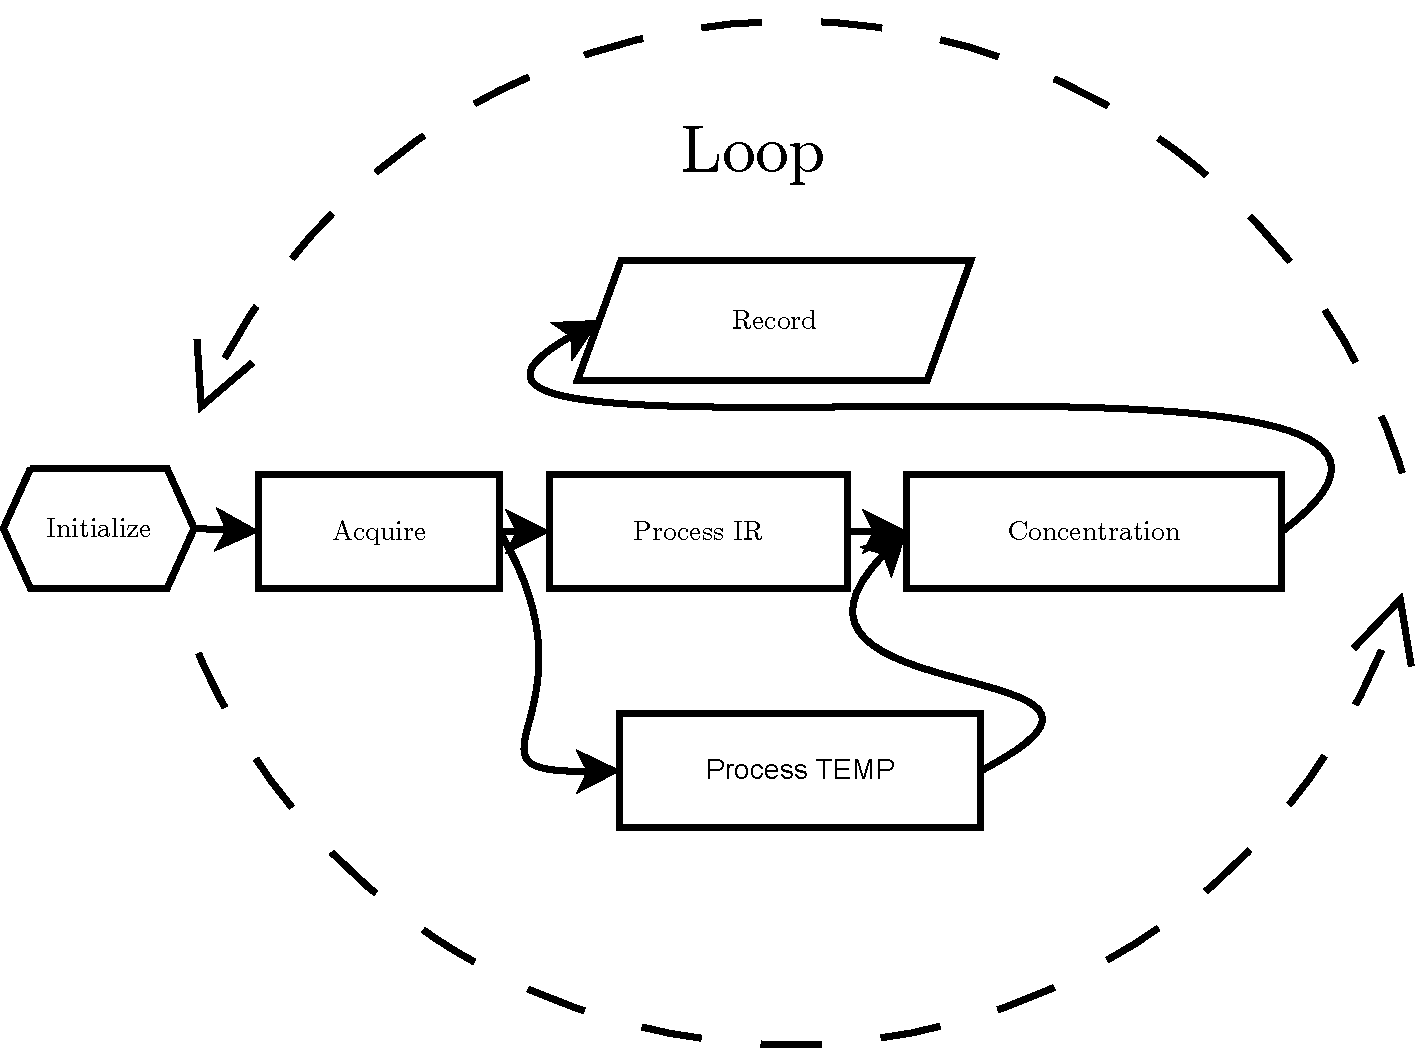
\includegraphics[width=\textwidth]{dataflow}
  \caption{Program dataflow chart. Arrows indicate direction of data flow,
    not dependance or sequentiality.}
  \label{fig:dataflow}
\end{figure}

\begin{figure}[htb]
  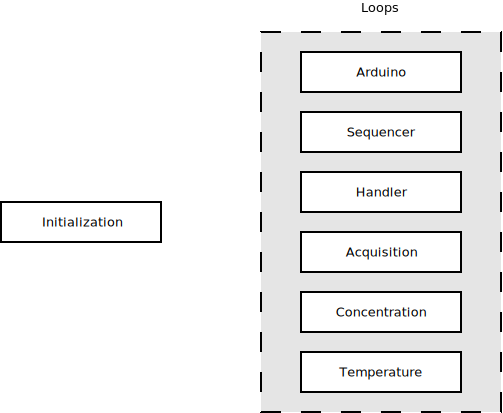
\includegraphics[width=\textwidth]{block-diagram-map}
  \caption{Block diagram functional components}
  \label{fig:block-diag-map}
\end{figure}

%Kirjallisuuviitteet
\bibliography{bibliography}
\bibliographystyle{unsrt}

\appendix
\appendixpage
\addappheadtotoc
\section{Directory listing}

\begin{tabular}{l l}
%% \hline
%% \multicolumn{1}{c} {Heading 1} & \multicolumn{1}{c} {Heading 2} \\
%\hline
\begin{minipage}{0.3\linewidth}\dirtree{%
.1 mims-project.
.2 data. 
.2 docs. 
.2 helpers. 
.2 test. 
.2 typedefs. 
.2 utilities. 
.2 main.vi. 
}\end{minipage}
&
\DTsetlength{0pt}{0pt}{0pt}{0pt}{0pt}
\begin{minipage}{0.7\linewidth}\dirtree{%
.1 Root directory.
.2 Contains sensor-configurations.ini.
.2 Documents related to the sensor hardware.
.2 Some helpfull functions.
.2 Unit \& other tests.
.2 Controls and clusters used by the program.
.2 Functions for performing more complex tasks.
.2 The main program.
}\end{minipage}
\\
%\hline
\end{tabular}

\end{document}
